% Template for a Computer Science Tripos Part II project dissertation
\documentclass[12pt,a4paper,twoside,openright]{report}

\usepackage{My_style}
\usepackage{dirtree}
\usepackage{multicol}
\usepackage{minted}
\usepackage[pdfborder={0 0 0}]{hyperref}    % turns references into hyperlinks
\usepackage[margin=25mm]{geometry}  % adjusts page layout
\usepackage{graphicx}  % allows inclusion of PDF, PNG and JPG images
\usepackage{verbatim}
\usepackage{docmute}   % only needed to allow inclusion of proposal.tex
\usepackage[utf8]{inputenc}
\usepackage{mathtools}
\usepackage{changepage}
\usepackage{url}
\usepackage{stmaryrd}
\usepackage{blindtext}
\usepackage{epigraph}
\usepackage{amssymb}

\usepackage{newunicodechar}
\usepackage{ifthen}

\newunicodechar{ℕ}{\ensuremath{\mathnormal {\mathbb{N}}}}
\newunicodechar{𝔹}{\ensuremath{\mathnormal {\mathbb{B}}}}
\newunicodechar{→}{\ensuremath{\mathnormal {\to}}}

\newunicodechar{⌞}{\ensuremath{\llcorner}}
\newunicodechar{⌟}{\ensuremath{\lrcorner}}
\newunicodechar{′}{\ensuremath{\prime}}
\newunicodechar{−}{\ensuremath{-}}
\newunicodechar{─}{\ensuremath{-}}
\newunicodechar{—}{\ensuremath{--}}
\newunicodechar{◆}{\ensuremath{\Diamondblack}}
\newunicodechar{⧫}{\ensuremath{\blacklozenge}}
\newunicodechar{∷}{\ensuremath{::}}
\newunicodechar{∙}{\ensuremath{\bullet}}
\newunicodechar{□}{\ensuremath{\Box}}
\newunicodechar{∎}{\ensuremath{\blacksquare}}
\newunicodechar{⋆}{\ensuremath{\star}}
\newunicodechar{●}{\scalebox{0.8}{$\bullet$}}
\newunicodechar{▸}{{\scalebox{0.7}{$\blacktriangleright$}}}


% indices
\newunicodechar{₀}{\ensuremath{_0}}
\newunicodechar{₁}{\ensuremath{_1}}
\newunicodechar{₂}{\ensuremath{_2}}
\newunicodechar{₃}{\ensuremath{_3}}

\newunicodechar{ₚ}{\ensuremath{_*}}
\newunicodechar{ₑ}{\ensuremath{_e}}
\newunicodechar{ᵢ}{\ensuremath{_i}}
\newunicodechar{ₖ}{\ensuremath{_k}}
\newunicodechar{ₘ}{\ensuremath{_m}}
\newunicodechar{ₙ}{\ensuremath{_n}}
\newunicodechar{ᵣ}{\ensuremath{_r}}
\newunicodechar{ₛ}{\ensuremath{_{\scriptscriptstyle \mathrm{S}}}}
\newunicodechar{ₓ}{\ensuremath{_X}}
\newunicodechar{ₗ}{\ensuremath{_l}}

\newunicodechar{₊}{\ensuremath{_+}}

% exponents
\newunicodechar{⁺}{\ensuremath{\textsuperscript{+}}}
\newunicodechar{⁻}{\ensuremath{\textsuperscript{-}}}

\newunicodechar{²}{\ensuremath{^2}}

\newunicodechar{ⁱ}{\ensuremath{^i}}


% ticks
\newunicodechar{′}{\ensuremath{'}}
\newunicodechar{″}{\ensuremath{'}}
% \newunicodechar{ˡ}{\ensuremath{^l}}
\newunicodechar{ᵐ}{\ensuremath{^{\scriptscriptstyle\mathrm{M}}}}
\newunicodechar{ʳ}{\ensuremath{^r}}
\newunicodechar{ᵒ}{\ensuremath{^o}}
\newunicodechar{ˢ}{\ensuremath{^s}}
\newunicodechar{ᶠ}{\ensuremath{^f}}
\newunicodechar{ᶜ}{\textsuperscript{c}}
\newunicodechar{ᵇ}{\ensuremath{^{\scriptscriptstyle\bo}}}
\newunicodechar{ᴮ}{\ensuremath{_*^{\scriptscriptstyle\bo}}}

\newunicodechar{ᴬ}{\ensuremath{^A}}
\newunicodechar{ᴵ}{\ensuremath{^I}}
\newunicodechar{ᴿ}{\ensuremath{^R}}
\newunicodechar{ᵀ}{\ensuremath{^T}}
\newunicodechar{ᵁ}{\ensuremath{^U}}
\newunicodechar{ⱽ}{\ensuremath{^V}}
\newunicodechar{ˡ}{\ensuremath{^{\scriptscriptstyle\Sigma}}}
\newunicodechar{ᴸ}{\ensuremath{^L}}
\newunicodechar{ᴹ}{\ensuremath{^{\scriptscriptstyle\mathrm{M}}}}


% Dots
\newunicodechar{⋯}{\ensuremath{\cdots}}

% Equality symbols
\newunicodechar{≡}{\ensuremath{\equiv}}
\newunicodechar{≢}{\ensuremath{\not\equiv}}
\newunicodechar{≟}{\mbox{\tiny\ensuremath{\stackrel{?}{=}}}}
\newunicodechar{≈}{\ensuremath{\approx}}

% Ordering symbols
\newunicodechar{≼}{\ensuremath{\preccurlyeq}}
\newunicodechar{≤}{\ensuremath{\le}}
\newunicodechar{⊑}{\ensuremath{\sqsubseteq}}
\newunicodechar{≥}{\ensuremath{\ge}}

% Arrows
\newunicodechar{→}{\ensuremath{\rightarrow}}
\newunicodechar{←}{\ensuremath{\leftarrow}}
\newunicodechar{⇒}{\ensuremath{\scriptstyle\Rightarrow}}
\newunicodechar{⇉}{\ensuremath{\rightrightarrows}}
\newunicodechar{↣}{\ensuremath{\funty}}
\newunicodechar{↝}{\ensuremath{\ren}}
\newcommand{\hackctxmap}[2]{\ctxmap{#1}}
\newunicodechar{⇝}{\hackctxmap}
\newunicodechar{⟶}{\ensuremath{\rightarrow}}
\newunicodechar{↦}{\ensuremath{\mapsto}}
\newunicodechar{↻}{\ensuremath{\circlearrowleft}}
\newunicodechar{⟿}{\ensuremath{\rightsquigarrow}}
\newunicodechar{◅}{\ensuremath{\triangleleft}}

% Mathematical symbols
\newunicodechar{∂}{\ensuremath{\partial}}
\newunicodechar{∋}{\ensuremath{\ni}}
\newunicodechar{∞}{\ensuremath{\infty}}
\newunicodechar{∀}{\ensuremath{\forall}}
\newunicodechar{∃}{\ensuremath{\exists}}
\newunicodechar{∄}{\ensuremath{\nexists}}
\newunicodechar{⊢}{\ensuremath{\vdash}}
\newunicodechar{⟨}{\ensuremath{\langle}}
\newunicodechar{⟩}{\ensuremath{\rangle}}
\newunicodechar{⊤}{\ensuremath{\top}}
\newunicodechar{∘}{\ensuremath{\circ}}
\newunicodechar{⊎}{\ensuremath{\uplus}}
\newunicodechar{×}{\ensuremath{\times}}
\newunicodechar{ℕ}{\ensuremath{\mathbb{N}}}
\newunicodechar{⟦}{\ensuremath{\llbracket}}
\newunicodechar{⟧}{\ensuremath{\rrbracket}}
\newunicodechar{∈}{\ensuremath{\in}}
\newunicodechar{↑}{\ensuremath{\uparrow}}
\newunicodechar{¬}{\ensuremath{\neg}}
\newunicodechar{⊥}{\ensuremath{\bot}}
\newunicodechar{↝}{\ensuremath{\leadsto}}
\newunicodechar{↶}{\ensuremath{\curvearrowleft}}
\newunicodechar{↺}{\ensuremath{\circlearrowleft}}
\newunicodechar{⊔}{\ensuremath{\sqcup}}
\newunicodechar{⨆}{\ensuremath{\bigsqcup}}
\newunicodechar{⋃}{\ensuremath{\bigcup}}
\newunicodechar{∩}{\ensuremath{\cap}}
\newunicodechar{∪}{\ensuremath{\cup}}
\newunicodechar{∅}{\ensuremath{\emptyset}}
\newunicodechar{∙}{\ensuremath{\cdot}}
\newunicodechar{∔}{\ensuremath{\app}}
\newunicodechar{⊗}{\ensuremath{\otimes}}
\newunicodechar{⊕}{\ensuremath{\oplus}}
\newunicodechar{⊖}{\ensuremath{\ominus}}
\newunicodechar{⊙}{\ensuremath{\FTens}}
\newunicodechar{⊸}{\ensuremath{\linto}}
\newunicodechar{⇾}{\ensuremath{\famto}}
\newunicodechar{⇨}{\ensuremath{\Rightarrow}}
\newunicodechar{′}{\ensuremath{'}}
\newunicodechar{〖}{\ensuremath{{\lwbrak}}}
\newunicodechar{〗}{\ensuremath{{\rwbrak}}}


% Misc
\newunicodechar{ℓ}{\ensuremath{\ell}}

% Greek uppercase
\newunicodechar{Δ}{\ensuremath{\Delta}}
\newunicodechar{Γ}{\ensuremath{\Gamma}}
\newunicodechar{Λ}{\ensuremath{\Lambda}}
\newunicodechar{Σ}{\ensuremath{\Sigma}}
\newunicodechar{Θ}{\ensuremath{\Theta}}
\newunicodechar{Ξ}{\ensuremath{\Xi}}
\newunicodechar{Ω}{\ensuremath{\Omega}}

% Greek lowercase
\newunicodechar{α}{\ensuremath{\alpha}}
\newunicodechar{β}{\ensuremath{\beta}}
\newunicodechar{δ}{\ensuremath{\delta}}
\newunicodechar{ε}{\ensuremath{\epsilon}}
\newunicodechar{φ}{\ensuremath{\phi}}
\newunicodechar{ϕ}{\ensuremath{\varphi}}
\newunicodechar{γ}{\ensuremath{\gamma}}
\newunicodechar{ι}{\ensuremath{\iota}}
\newunicodechar{κ}{\ensuremath{\kappa}}
\newunicodechar{λ}{\ensuremath{\lambda}}
\newunicodechar{μ}{\ensuremath{\mu}}
\newunicodechar{ψ}{\ensuremath{\psi}}
\newunicodechar{η}{\ensuremath{\eta}}
\newunicodechar{ρ}{\ensuremath{\rho}}
\newunicodechar{ϱ}{\ensuremath{\varrho}}
\newunicodechar{σ}{\ensuremath{\sigma}}
\newunicodechar{ς}{\ensuremath{\varsigma}}
\newunicodechar{τ}{\ensuremath{\tau}}
\newunicodechar{ξ}{\ensuremath{\xi}}
\newunicodechar{χ}{\ensuremath{\chi}}
\newunicodechar{ζ}{\ensuremath{\zeta}}
\newunicodechar{Π}{\ensuremath{\Pi}}
\newunicodechar{ω}{\ensuremath{\omega}}
\newunicodechar{ƛ}{\ensuremath{\boldsymbol{\lambda}}}

\newunicodechar{ℐ}{\ensuremath{\Ind}}

% Macros

\newcommand{\agdacode}[2][CoreL]{\begin{spacing}{1.1}%
\ExecuteMetaData[formalisation/agda/latex/#1.tex]{#2}%
\end{spacing}}
\newcommand{\aty}[2]{\AgdaBound{#1}\,\AgdaSymbol{:}\,\AgdaDatatype{#2}}

\newcommand{\Actxmap}[3]{#1\AgdaSpace{}%
\AgdaOperator{\AgdaFunction{–[}}\AgdaSpace{}%
\AgdaBound{#2}\AgdaSpace{}%
\AgdaOperator{\AgdaFunction{]→}}\AgdaSpace{}%
#3}



%%%%%%%%%% AGDA ALIASES

\newcommand{\APT}{\AgdaPrimitiveType}
\newcommand{\AK}{\AgdaKeyword}
\newcommand{\AM}{\AgdaModule}
\newcommand{\AS}{\AgdaSymbol}
\newcommand{\AStr}{\AgdaString}
\newcommand{\AN}{\AgdaNumber}
\newcommand{\AD}{\AgdaDatatype}
\newcommand{\AF}{\AgdaFunction}
\newcommand{\AR}{\AgdaRecord}
\newcommand{\ARF}{\AgdaField}
\newcommand{\AB}{\AgdaBound}
\newcommand{\AIC}{\AgdaInductiveConstructor}
\newcommand{\AO}{\AgdaOperator}
\newcommand{\AUS}{\AgdaUnderscore{}}
\newcommand{\AG}{\AgdaGeneralizable}
\newcommand{\AAr}{\AgdaArgument}
\newcommand{\AInd}{\AgdaIndent}


%\raggedbottom                           % try to avoid widows and orphans
\sloppy
\clubpenalty1000%
\widowpenalty1000%

\renewcommand{\baselinestretch}{1.1}    % adjust line spacing to make
                                        % more readable

\begin{document}
\pagenumbering{gobble}

\newcommand{\mcandidate}{UNCLEAR}
\newcommand{\mfullname}{Patrick Nickols}
\newcommand{\mcollege}{Downing College}
\newcommand{\mtitle}{Formalising PCF and its Denotational Semantics in Agda}
\newcommand{\mexamination}{Computer Science Tripos -- Part II}
\newcommand{\mdate}{TBD}
\newcommand{\moriginator}{Mr Dima Szamozvancev}
\newcommand{\msupervisor}{Mr Dima Szamozvancev}
\newcommand{\mwordcount}{TBD}
\newcommand{\mlinecount}{TBD}
% Consent to the dissertation made available to University members
\newcommand{\mconsent}{I am content for my dissertation to be made available to the students and staff of the University.}
% For the Declaration of originality
\newcommand{\msignature}{Patrick David Nickols}

\bibliographystyle{plain}


%%%%%%%%%%%%%%%%%%%%%%%%%%%%%%%%%%%%%%%%%%%%%%%%%%%%%%%%%%%%%%%%%%%%%%%%
% Title


\thispagestyle{empty}

\rightline{\LARGE \textbf{\mfullname}}

\vspace*{60mm}
\begin{center}
\Huge
\textbf{\mtitle} \\[5mm]
\mexamination \\[5mm]
\mcollege \\[5mm]
\mdate  % today's date
\end{center}

%%%%%%%%%%%%%%%%%%%%%%%%%%%%%%%%%%%%%%%%%%%%%%%%%%%%%%%%%%%%%%%%%%%%%%%%%%%%%%
% Proforma, table of contents and list of figures

\pagestyle{plain}

\newpage
\newpage
\section*{Declaration of originality}

I, \mfullname{} of \mcollege, being a candidate for Part II of the Computer Science Tripos, hereby declare that this dissertation and the work described in it are my own work, unaided except as may be specified below, and that the dissertation does not contain material that has already been used to any substantial extent for a comparable purpose. \mconsent

\bigskip
\leftline{Signed \msignature}
\bigskip
\leftline{Date \today}

\chapter*{Proforma}

{\large
\begin{tabular}{ll}
Candidate Number:   & \bf \mcandidate                   \\
Project Title:      & \bf \mtitle                       \\
Examination:        & \bf \mexamination, \mdate         \\
Word Count:         & \bf \mwordcount\footnotemark[1]   \\
Code Line Count:    & \bf \mlinecount \footnotemark[2]  \\
Project Originator: & \bf \moriginator                  \\
Supervisor:         & \bf \msupervisor                  \\ 
\end{tabular}
}
\footnotetext[1]{This word count was computed
by \texttt{detex diss.tex | tr -cd '0-9A-Za-z $\tt\backslash$n' | wc -w}
}
\footnotetext[2]{This code count was computed
by \texttt{find . -name "*.agda" | xargs wc -l}
}
\stepcounter{footnote}


\section*{Original Aims of the Project}
% At most 100 words

TODO


\section*{Work Completed}
% At most 100 words

TODO

\section*{Special Difficulties}
% At most 100 words

TODO

\newpage

\tableofcontents

\listoffigures

\newpage
\section*{Acknowledgements}

TODO

%%%%%%%%%%%%%%%%%%%%%%%%%%%%%%%%%%%%%%%%%%%%%%%%%%%%%%%%%%%%%%%%%%%%%%%
% now for the chapters

\pagestyle{headings}
\chapter{Introduction}
\section{Motivation}
\pagenumbering{arabic}
\epigraph{Beware of bugs in the above code; I have only proved it correct, not tried it.}{--- \textup{Donald Knuth}}

Everyone who writes code frequently has written buggy code. The costs of these errors vary from minor decreases of self-esteem on the behalf of the programmer to large financial losses (CITE HERE) and, in some cases, deaths (CITE HERE). Programmers have year after year been flummoxed by increasingly unpredictable errors, as programs grow too complicated to easily reason about, but too useful to discard. Various approaches have been suggested to deal with this, and one calling out from those with a mathematical background is formalisation - defining precisely what it is that programs can and should do. This specification of the ``meaning" of a language and its programs is called ``semantics"\footnote{This term comes to the computer science community from linguistics, where its meaning is similar. The study of the semantics of a spoken language is the study of its words and sentences' meanings.}. 

While this seems an attractive idea, there are clear problems with backpatching formalisation onto existing languages. C, whose applications power most of the modern technological world, \textit{does not have a formal semantics}\cite{C-semantics}, while producing a parse tree for C++ \textit{is undecidable}\cite{C++-undecidable}, which implies its semantics are severely underspecified. 

The challenge then, is finding a middle ground between useless formalisation of unimportant concepts in impractical languages, and the impossibility of formalising the most relevant concepts in the most relevant languages. 

\section{Background}
\subsection{(Denotational) Semantics}
After one decides it's worth trying to formalise what a language means and what its programs do, there are several approaches, which are generally said to fall into one of three categories (Footnote about who agrees there are 3 main ones).

\textit{Axiomatic Semantics} reasons in terms of precondition and postconditions: assertions that are true before some code is run and the corresponding assertions that must be true after accordingly.

\textit{Operational Semantics} describes how programs transform as they are run in terms of a reduction relation\footnote{With deterministic small-step reduction, we hope that the reduction relation is a function, i.e. that each term reduces in at most one way.} saying that e.g. \texttt{if true then x else y} reduces to \texttt{x}. This approach is to some extent implictly required by anyone creating a programming language. While it may not be formalised and precise, to invent a programming language, one needs to impart meaning to its keywords, and thus have a mental model of what each operation does. 

\textit{Denotational Semantics} aims to find a correspondence between programs and mathematical objects, with the hope being that one can reason about the objects more easily, using tools from mathematics. Ideally the correspondence is meaningful in mathematically provable ways\footnote{For example, we hope if that if a term reduces via the operational semantics to another term, their denotations are related in some way (in fact, we normally want equality between the two terms). This property is called soundness and is detailed more later.}. It is this approach that I will be following. 

While this may sound abstract, I claim that in certain cases this is obvious and even done implicitly: the common mental model for a programming language's integer type is the set $\mathbb{Z}$\footnote{In reality, many languages don't support arbitrary integers in their int type, but a restricted class. In this case the mental model may be a subset of $\mathbb{Z}$.}. The question in this case becomes what to do when things are not obvious, or the obvious thing fails? We can view product types as corresponding to (cartesian) products of sets, and functions to functions, but what then does \texttt{while} correspond to? And how do we know that our chosen interpretation is effective and useful? These are the sorts of questions that the denotational semantics course \cite{Course} aims to answer. One level higher, the course's answers are the questions that this dissertation aims to formalise. 
\subsection{PCF}
Programming Computable Functions, (from here on PCF), is a toy programming language created by Dana Scott in 1969 \cite{Scott} for the express purpose of defining a denotational semantics. It is thus small, but sufficiently non-trivial that defining its semantics could yield a publishable paper\footnote{In fact, the cognoscenti will note that this skims over some important details. The paper was not concerned with a programming language PCF, but merely a logical system (which Scott called LCF). Scott was seeking an alternative to the lambda calculus as a model of computation. It was extended to a programming language in several years later by Plotkin \cite{Plotkin}.}. Slightly different versions of it exist in the literature; I will use the modern\footnote{In particular, Scott avoided lambdas (he thought substitution theorems were a pain!), and had K and S combinators instead.} one (almost exactly) as defined in the course. While we later examine its terms and types precisely in chapter 2, it is a good approximation to think of it as a variant on the simply-typed lambda calculus, with ground types of booleans and integers, and the basic corresponding operations (if-expressions, a test-for-zero, the successor and predecessor functions). 

The defining feature of PCF, which leads directly to the denotational objects chosen to represent its terms is the fixpoint operator. Given a function $f : A \to A$, we have $\text{fix}(f) = f (\text{fix}(f))$ (where $=$ is being used approximately). That is the fixpoint of $f$ is an input to $f$ whose output is itself, i.e. a fixed point of $f$. From a practical point of view, this allows us to implement recursion: e.g. to define $f(n) = n!$ we can write\footnote{in an approximate notation, the details of language syntax are not the point here.}
\[
\text{fix}\left( \lambda f : \text{nat} \to \text{nat}. \lambda n: \text{nat}. \text{if } n = 0 \text{ then } 1 \text{ else } n * f (n-1)\right).
\] This is analogous to the $Y$-combinator of the untyped lambda calculus. However, the untyped lambda calculus is a pathological language, where any term can be an input to any function\footnote{Scott wrote that the untyped lambda calculus ``makes no sense whatsoever".} and every function has a fixed point. It is thus perhaps surprising that in PCF, where we have types and slightly ``better behaviour", we still expect every function to have a fixpoint. What, one may ask, should the fixpoint of the successor function be, given that clearly we don't have any $n$ such that $n+1 = n$? 

It is exactly this question: ``what mathematical objects guarantee us that all functions have fixed points?" that led Scott to his chosen semantics of domains and continuous functions\footnote{In fact, the avid historian may take issue with this characterisation. Scott's paper discusses the difficulties of simulating partial functions with total functions, and says that stumbling upon domains was mainly a consequence of trying to represent undefined behaviour with the extra element $\bot$. That everything ends up working out so nicely with the fixed point operator he attributes to luck.}.

 

\section{Project Description}
The aim of the project was to formalise the main results of the Denotational Semantics course. In particular, from the first half of the course, I wanted to formalise:
\begin{itemize}
\item Lambek's Lemma (that the least pre-fixed point is itself a fixed point)
\item Tarski's fixed point theorem
\item The continuity of the fixpoint operator.
\end{itemize}
And from the second part of the course, concerning PCF and its denotation, I wanted to formalise:
\begin{itemize}
\item The language PCF itself
\item Its denotational semantics
\item A progress theorem (that well-typed terms don't get stuck, they are either values or can reduce)
\item A preservation theorem (that terms have the same type before and after reduction)
\item A soundness theorem for its semantics (that if one term reduces to another, then they have the same denotation).
\end{itemize}
Extensions that I considered at the time of proposing were:
\begin{itemize}
\item A category-theoretic perspective on the same material
\item A compositionality theorem (that if two terms have the same denotation, all contexts with one swapped for the other also have the same denotation)
\item An adequacy theorem (that for ground-typed terms, if they have the same denotation, one reduces to the other). 
\item Scott induction (a specific induction principle when dealing with the fixed point operator). 
\end{itemize}
Of these, I tackled the second and fourth.
\section{Related Work}
The most relevant work being produced in the last few years has come primarily from the UK, notably the research group of Birmingham, involving work by Escardo, De Jong, and Hart. However, their work, while attacking the same or similar problems (also in Agda), answers these questions via the lens of Homotopy Type Theory. This is an abstract approach primarily motivated by Voevodsky, that has been working to reshape mathematics' underpinnings, avoiding ZFC as a foundational model, and instead aiming at type-theoretic primitives\footnote{This effort primarily intensified between 2012 and 2013, when the Institute for Advanced Study held ``A special year on Univalent Foundations in Mathematics": a year dedicated to advancing and propogating the spread of this thinking.}. I will not dwell too much on its details but the curious reader is invited to Hart's work \cite{Hart}, but note that this approach is different in motivation and direction from my project\footnote{In particular, ???}, though we prove some of the same theorems.

Beyond that, Streicher \cite{Streicher} covers much of the material , but with a pen-and-paper approach while Wadler \cite{PLFA} covers using Agda as a proof assistant, and implementing a PCF-like language, but does not implement its denotational semantics\footnote{He instead implements a denotational semantics for the untyped lambda calculus.}. Finally I am indebted to my supervisor's former student's dissertation \cite{Ted}, as an example of how to write a Cambridge Part II Dissertation with an Agda project: although we proved quite different things, there are heavy motivational overlaps. 
\chapter{Preparation}
\section{PCF}
\subsection{Syntax}
The variant of PCF we will be considering looks much like a simply-typed lambda calculus with a few ground terms and primitives, and the key extra feature of a fixpoint operator. Its grammar is defined by (where $\mu$ is the fixpoint operator and $x$ is a fresh variable name\footnote{Although, since we will use de Bruijn indices, this is just a visual aid.}):
\[
L, M, N := x \mid \text{Zero} \mid \text{True} \mid \text{False} \mid \lambda x: \tau . M \mid M \cdot N 
\]
\[
\text{Succ }M \mid \text{Pred }M \mid \text{Is-Zero }M \mid \text{If }L \text{ then }M \text{ else }N \mid \mu M
\]
\subsection{Typing Relation}
The typing relation is unsurprising. We have a type of naturals, a type of booleans, and function types. Note in particular that because of design decisions in implementation, we will only deal with well-typed terms.
\[
\tau, \tau' := \mathbb{N} \mid \mathbb{B} \mid \tau \to \tau'
\]
\subsection{Notable Features}
PCF is Turing complete. This is a well-known result, and its proof is expressed in the lecture notes. It relies upon the lemma that partial recursive functions are Turing-complete. We then show that we can encode partial recursion in PCF, and are thus done. The key details are that we have natural numbers, the fixpoint operator and case-destructors for integers - equivalent forms of PCF have a case matching on integers with $0$ and suc($n$) that suffices as well\footnote{C.f. e.g. \cite{PLFA}}. 

A perhaps surprising result is that the fixpoint operator (which allows unbounded recursion) is not sufficient on its own: in the simply typed lambda calculus augmented with only the Y combinator, everything, in particular whether a program terminates, is decidable. Details can be found in Statman's work \cite{Statman}. 
\subsection{Relation to other languages}
A natural question to ask, and a common refrain from those who work on more applied subjects is something along the lines of ``What's the point? Are you really proving anything if you only deal with toy languages?". However these concerns can be addressed in two ways. Firstly, it should be noted that progress is incremental: it was easier to give an operational semantics for languages that closely model the typed lambda calculus than for C, but seeing an operational semantics for the typed lambda calculus makes providing one for C much more feasible. 

Secondly, and of some importance for the PCF-interested reader: PCF was the inspiration behind ML and thus OCaml, F\# etc. In particular, Milner developed ML for a theorem-proving system based on LCF. Proving things about PCF can thus be viewed as foundational work for proving things about languages like OCaml, Haskell and F\#.
\section{Agda}
\subsection{Curry--Howard}
The Curry--Howard correspondence is undoubtedly one of the most intriguing connections between logic and computer science. While it may not seem surprising that product types correspond to conjunctions, who could have foreseen that call-by-name is de-Morgan-dual to call-by-value \cite{Ted}, or that classical logic corresponds to the \texttt{call/cc} construct in Scheme \cite{Call-cc}?

I will not dwell on the details here, but the key theme of the generalised Curry-Howard correspondence is that types correspond to propositions. The result is that proving a theorem holds can be done by creating an object of the correct type in a programming language. For example, to prove that $A \implies B$, we can instead create a function from a type corresponding to $A$ to a type corresponding to $B$. 

It is exactly this feature that we will exploit of Agda. Agda is ostensibly a programming language, similar in spirit and history to Haskell, with its main value proposition being dependent types and good editor support for use as a theorem prover. However, the reason it works as a theorem prover is not because Agda has some datatype called ``theorem" and corresponding semantics for proving them, but simply because of the Curry--Howard correspondence. In addition, the use of dependent types allows for easy translation of first-order-logical statements with universal quantification. 

An example may be instructive. (STILL TO DO OR TO REMOVE).
\subsection{Dependent Types}
When exploring the Curry-Howard correspondence, there are two ways of trying to better understand it and extend it. One is to look at existing programming languages, and see if any features correspond to aspects of logic that have not yet been accounted for. The other, and the source of dependent types, is to look at logic and see what features of logic could be added to a programming language. After Curry \cite{Curry-Howard} recognised the link between intuitionistic logic and functions (e.g. of the simply-typed lambda calculus), decades later Howard\footnote{This is unimportant to the student of computer science, but a remarkable characterisation of the time he and his colleague Anil Nerode spent at UChicago can be found on the web (CITE).} \cite{Howard} and de Bruijn considered how to extend the simply-typed lambda calculus to model universal and existential quantification. The result was the invention (or discovery) of dependent types.

Informally, dependent types extend a type system by allowing types to depend not only on other types (as e.g. a function from $A$ to $B$ depends on $A$ and $B$), but also on values. 

Formally, there are two constructs we wish to consider. The dependent product\footnote{The terminology here is exceedingly confusing and inconsistent. There are good arguments for calling either of the constructs we consider a dependent product. One can only hope the field crystallises around one of the two opposing terminologies. This object is also called a dependent function, as it is a generalisation of a function.} is a function from a type $A$ to a type that depends on the value of the input. Agda's syntax, which reflects this is: $(a : A) \to B(a)$, where $B(a)$ is a type. $B$ is not therefore a type, but a function from $A \to U$ where $U$ is a ``universe" of types\footnote{The pedantic Russell-paradox fan may be disappointed by this dissertation. I will try to avoid all mention of Grothendieck universes, save where completely necessary, but note that this is a choice, and these considerations do matter. They are just not the main point I am aiming at here}. That is, for every $a \in A$, $B(a)$ is a type. This family of types $B$ may be called a dependent type\footnote{Again, terminology is inconsistent. People may instead call $B(a)$ a dependent type}. The notation people use more widely (outside of Agda) for this function from $A$ to $B(a)$ is:
\[
\prod_{a: A} B(a).
\]
When $B$ is a constant function, i.e. $B(a)$ is a specific type independent of $a$, then this is just a familiar type $A \to C$ where $C = B(a)$.

The other construct is the dependent sum\footnote{Elsewhere, the ``dependent product", as it is a tuple, and tuples are products.}. A dependent tuple is a pair, where (reusing the example types and families), the first element $a$ is of some type $A$ and the second element of type $B(a)$. This enables us to encode (constructive) existentials, where  we wish to show there is an $a$ that satisfies $B(a)$ (e.g. there is a prime integer whose digits sum to 47) and a proof that it satisfies. Agda's standard library has a function with the following type signature:
\begin{minted}{agda}
(x : A) → B a → ∑ A B.
\end{minted} 
Morally this type is $(a : A) \times B(a)$, but for it to work in Agda the standard library declares a new datatype $\Sigma$ which takes two arguments, but in curried form, and combines them into a pair. Where $B$ is constant, and so $B(a) = C$ for all $a$, this is just the familiar type of $A \times C$. The mathematical notation employed is
\[
\sum_{a : A} B(a). 
\]
\subsection{Using Agda}
Despite being ostensibly a functional programming language with dependent types, Agda's interactive IDE features are optimised for theorem-proving. The following quality-of-life features should not be underestimated, they can save countless hours and greatly reduce the number of levels of abstraction the working programmer need deal with at one time. My favourite feature of Agda is the ability to put in ``holes" in ones code. By putting a \texttt{?}, the IDE will put in an interactive box that, via solving unifications, knows what type it must have (if it can be deduced). This makes scaffolding one's code easier, as one can write the obvious bits and leave the tricky parts (like de Bruijn index manipulations) in a hole. In addition, holes can be auto-filled if the unification allows a unique solution, or can be randomly filled by something of the correct type (which in sufficiently restrictive type systems is often the correct term). 

Secondly, one can case match on constructors. This makes the category of precise but uninteresting proofs that can come up during programming language research much more manageable\footnote{Paulson \cite{Larry} describes these proofs as ``conceptually trivial but extremely tedious". They are one of the best parts of formalising, in that they can be genuinely easier to write on a computer than by hand.}. When one does induction on a relation, one needn't check all the reduction steps, one can just use a hotkey to autopopulate the needed steps. 
\section{Software Engineering}
\subsection{Starting Point}
The main project that is most similar to this is Hart's \cite{Hart}, but I did not look at that code until after writing my own, to avoid retracing the same steps, and due the different spirits of our pursuits. I wished to formalise a lecture course, whereas his project is an extension to a larger goal of unifying all of mathematics with constructive Homotopy Type Theory as the basis.

The two most relevant courses (both began after the disseration) in the Tripos are, of course, \textit{Denotational Semantics} and \textit{Type Theory}. The most relevant part of \textit{Type Theory} was an introduction to Agda and dependent types, but as this was at the end of the lecture series, I had to pre-study this, in order to start working in good time. Several lectures from the Part III unit of Assesment \textit{Category Theory} cover denotations of the lambda calculus in a Cartesian-closed category, and these were also very relevant. 

Before this project, I had little experience formalising proofs. I had experimented with the natural numbers game \cite{NatNums} which is based on Coq, a similar, but more tactic-based dependent-type theorem prover. However, after project choice, I began completing exercises from PLFA \cite{PLFA} over the summmer, to acquire some familiarity with the syntax and IDE-features of Agda. In particular, the formalisation of the language of a PCF-like language and its operational semantics in PLFA was extremely useful to me, although this represented a small part of my project.
\subsection{Methodology}
Much like learning mathematics is iterative, and learning new things requires mastering prior material, so too is formalising. While Agda does allow holes, it is very difficult to make further progress without finishing prior work. For example, without defining what the lub of a flat chain is, it is almost impossible to prove any theorems about them. This is quite different from standard software development, in which more things can be worked on concurrently and adjusted, as parts are more decomposable, and dependencies are often structured less vertically. The consequence is that standard software engineering methodologies, like agile development, are inappropriate here. I initially established what I wanted to formalise in Agda, and then worked on each goal one by one, until done. This model therefore is closest to the waterfall method, where a full requirements analysis was conducted, then work was produced. The difference is that due to Agda's type checker, the verification was integrated with the implementation, each proof could be checked as it was written, rather than separating the verification from the implementation. 
\subsection{Tools and Design}
I used Emacs \cite{Emacs} as it is often said to be the editor with the best Agda support \cite{PLFA}. I had little experience with Emacs but had some with Vim and so consequently installed EVIL-mode \cite{Evil} to smoothen this transition. The dissertation itself was produced in \LaTeX. Both the source code for the project and for the \LaTeX-writeup are stored on a Git repository (hosted on Github), along with the exploratory work I did on PLFA over the summer. Snapshots of the Git repository at important milestones (e.g. the proof of Tarski's fixed point theorem) have been taken on a separate PC, in case of Git-related emergency. 
\subsection{Requirements Analysis}
I performed a MoSCoW requirements analysis before beginning. I concluded:

Must haves:
\begin{itemize}
\item The objects of domain theory: domains, chains, least fixed points, continuous functions etc.
\item Tarski's fixed point theorem.
\item Lambek's lemma.
\item The continuity of the fixpoint operator.
\item PCF in Agda, with its operational semantics.
\item A progress theorem for PCF.
\item A preservation theorem for PCF.
\item Denotational semantics for PCF.
\item A soundness theorem for PCF, relating its denotational and operational semantics.
\end{itemize}
Should haves:
\begin{itemize}
\item Scott induction.
\end{itemize}
Could haves:
\begin{itemize}
\item An adequacy theorem for PCF's denotational semantics.
\item A category-theoretic perspective on the material.
\item A compositionality theorem for PCF's denotational semantics.
\end{itemize}
Won't haves:
\begin{itemize}
\item Anything about performance/timing of code.
\item Anything to do with full abstraction.
\end{itemize}
\chapter{Implementation}
\section{Overview}
The entire body of the dissertation's coding work can be found here (LINK) and is in a directory structured like so:
\dirtree{%
.1 Diss.
.2 misc.agda.
.2 DomainTheory.
.3 BasicObjects.
.4 posets-etc.agda.
.4 theorems.agda.
.3 ContinuousFunctions.
.4 if-cont.agda.
.4 cur-cont.agda.
.4 ev-cont.agda.
.4 fix-cont.agda.
.2 PCF.
.3 pcf.agda.
.3 progress.agda.
.3 soundness.agda.
.3 soundness-lemmas.agda.
}
\vspace{5mm}
Note that this is a stylistic choice that was made to suit code modularity and organisation, in keeping with professional software engineering practice. The obvious choice that initially seemed somewhat attractive, given the dissertation being a formalisation of a lecture series, was to structure the code after the course i.e. a file of ``theorems from lecture 1", ``theorems from lecture 2" etc. This is impractical for multiple reasons however: not only does it make it hard to navigate (one needs to remember which lecture each theorem was proved in), but it also makes it much harder to track dependencies, as the course is taught in a way optimised for student learning, rather than trying to have every lemma proved next to the theorem it is used in. 

This chapter will serve as a ``tour" of the repository. Obviously, excessively technical deep dives into particulars will not be appropriate, but I will try to highlight interesting cases of theorems or technology or design considerations, both from the perspective of the pen-and-paper theorem prover, and the Agda programmer. 

\section{The basic objects of domain theory}
\subsection{A note about aesthetics}
Agda is a beautiful programming language in which to formalise mathematics. Two particular features stick out from an aesthetic point of view: it allows mixfix notation, and in common text-editors it has good support for inputting mathematical Unicode characters (using a \LaTeX-like syntax). While aesthetics are nebulous and hard to quantify, the benefits of these features should not be written off. Consider the first ``definitional" slide\footnote{This is the 15th slide of the course. The first lecture is dedicated to motivating the field, rather than providing any technical definitions} of the lecture course \cite{Course}.
\begin{center}
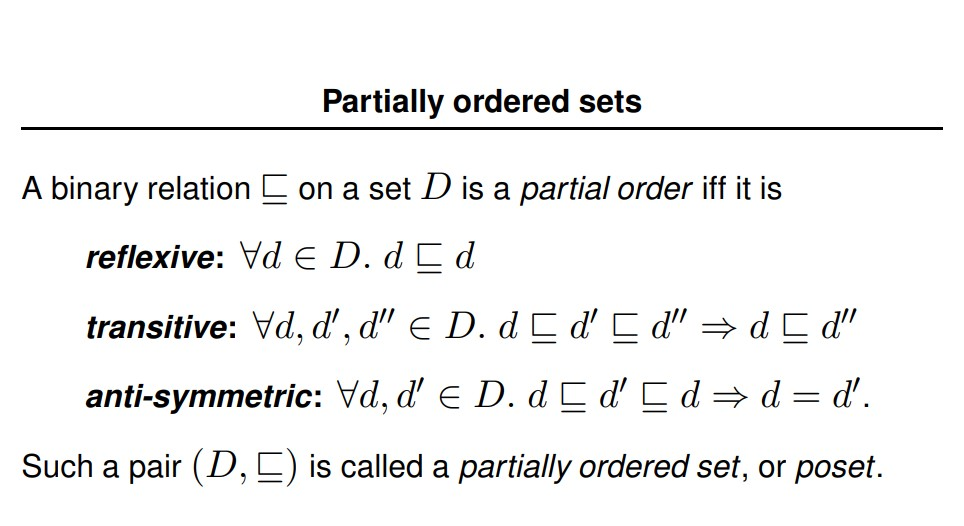
\includegraphics[scale = 0.7]{figs/poset_def}
\end{center}

The corresponding Agda code looks as follows:
\begin{minted}{agda}
record poset (D : Set) (_⊑_ : D → D → Set) : Set where
  field
    reflexive     : ∀ {d : D} → d ⊑ d 
    transitive    : ∀ {d d′ d'' : D} → (d ⊑ d′) → (d′ ⊑ d'') → (d ⊑ d'')
    antisymmetric : ∀ {d d′ : D} → (d ⊑ d′) → (d′ ⊑ d) → d ≡ d′
\end{minted}
This similarity was a key aim of my project. One of the main benefits of proof formalisation is that it massively narrows what one must trust (Cite/footnote talia ringer). To know that my Agda code is correct, one doesn't need to take it on faith, only that Agda's type-checker itself is correct. With that assumption, the code's correctness follows logically from the fact it type checks. However, this sounds very convenient, but it is very easy to prove things in Agda that are true, but not what you are trying to prove, or to be unable to prove things that are true. Therefore, to properly understand what it is that code is trying to prove and whether it succeeds, it is not only important that one's code type-checks, but also that it can be visibly seen to have type signatures corresponding to the intended theorems. 

For example, I may try to prove that all posets have a least element\footnote{This example is not a theorem. For example, the integers under the normal ordering relation do not have a least element.} and I may conceivably create a function in Agda whose type signature is:
\begin{minted}{agda}
poset-least-element : {P : Set} {⊑ : P → P → Set} (P⊑ : poset P ⊑) → least-element P
\end{minted}
That is a function which takes a poset (with underlying set P and relation ⊑) and returns a least element of P. Since in Agda all functions terminate and are total, the function corresponding to this type signature (if it typchecks) is a proof that all posets have least elements.

But, the important point here has a symmetry with the point of denotational semantics. The map is not the territory and the \texttt{least-element} record defined in Agda may not accurately represent what a least element of a set really is. So, knowing that code type checks and thus that theorems' proofs are valid in Agda, is only good in so far as one trusts that the objects in question are encoded correctly. This corresponds to the difference between verification (checking that an object matches its formal specification) and validation (checking that a formal specification matches what is actually desired). The typechecker can handle verification, but it is up to the Agda programmer to try to make validation doable by eye. 

It was thus a key aim of my project to encode the objects not just correctly but obviously so, as far as possible: the closer to the course's definitions (both in content and notation), the more confident the reader can be that the \texttt{poset} in my code is the same as in the lectures and the wider study of posets. 

This is not as straightforward as it sounds however, as this task directly clashes with the process of formalisation. Often the representation chosen in lectures for ease of student understanding is not as easy to work with and may lead to later difficulties. To try to illustrate the range of ways of representing things, both in Agda, and mathematically, there will be two case studies, I will highlight both chains and posets, but note that for most objects, similar thoughts and issues arise. 
\subsubsection{Posets}
A poset is defined in the course\footnote{and everywhere else, this is a well-agreed-upon term. C.f. ``domain" or ``PCF" which differ in definition depending on author.} as a set, a relation on that set and some properties of that relation. Agda's basic syntax for defining novel types has two options. One can define a datatype with corresponding constructors (similar to ML-derived languages), or one can define records. Records are simply product types with named fields, each of which has its own type. 

Since posets have no reason to need more than one constructor, the record seems a better option. 

But, even then, choices remain. Records are parameterised: that is, they may take inputs (via their type) that are not one of their fields. It is not always clear what belongs as a parameter, and what belongs as a field in a record. Thus, rather than the above definition, we could instead define analogously (footnote about Grothendieck universes):
\begin{minted}{agda}
record poset : Set where
  field
    A : Set
    R : A → A → Set
    reflexive     : ∀ {d : D} → d ⊑ d 
    transitive    : ∀ {d d′ d″ : D} → (d ⊑ d′) → (d′ ⊑ d″) → (d ⊑ d″)
    antisymmetric : ∀ {d d′ : D} → (d ⊑ d′) → (d′ ⊑ d) → d ≡ d′
\end{minted}

Or, we could instead say that a poset is a set with a partial order on that set. This could lead to:
\begin{minted}{agda}
record partial-order (A : Set) : Set where
  field
    R : A → A → Set
    reflexive     : ∀ {d : D} → d ⊑ d 
    transitive    : ∀ {d d′ d″ : D} → (d ⊑ d′) → (d′ ⊑ d″) → (d ⊑ d″)
    antisymmetric : ∀ {d d′ : D} → (d ⊑ d′) → (d′ ⊑ d) → d ≡ d′
record poset : Set where
  field
    A  : Set
    po : partial-order A
\end{minted}

These choices may seem relatively inconsequential, but indeed not only do such choices affect the ease of writing and reading the code that results, but they can make some ideas almost impossible to express (or relatively easy). Note for example, that in our first choice of implementing \texttt{poset} where the set and relation are parameters, there is no type of posets generally, and in fact all posets of the same type (i.e. sharing the same underlying set and relation) are essentially the same. 

Thus, if we wish to quantify over all posets, we need to first quantify over all sets, all corresponding relations, and then over all posets with the bound set variable, and bound relation variable. This approach does not seem too harmful at first, but quickly becomes almost insurmountable if one chooses to follow it. The interested reader is invited to (CITE OLD COMMIT) where one can see my code which originally took this approach. The theorems I wished to prove quickly became difficult to even provide the type signature for, let alone the actual proofs. For example, in an ideal world, to provide a type signature for a fixpoint operator that takes a function, and returns its least prefixed point, one might hope to write:
\begin{minted}{agda}
fixpoint : (A : domain) → (f : A → A) 
  → continuous-function f 
  → least-pre-fixed f
\end{minted}
or even just:
\begin{minted}{agda}
fixpoint : continuous-function → least-pre-fixed
\end{minted}
where the actual definition of $f$ (and hence its domain and codomain) is included in the record. However, note that this is an example of where representation matters. We cannot take fixpoint of every continuous function, only continuous endofunctions. Thus, we want a way to quantify over these functions.

However, if one needs to quantify over posets to do so, one might then need to quantify over the underlying sets of these posets (if they are parameters) and since a function has a domain and a codomain, this would require even more quantifying variables, and the type signature may become massively confused, to something like\footnote{This is a real example, with the name of the function changed}
\begin{minted}{agda}
fixpoint : (D : Set) (_⊑_ : D → D → Set) 
    (P : poset D _⊑_) (⊥ : D) (P′ : domain P ⊥) (f : D → D) 
    (cont-fun : continuous-fun P P f) 
  → least-pre-fixed P f
\end{minted}

This becomes unwieldy quickly. 
\subsubsection{Chains}
The difficulty of defining posets is mostly artificial, and introduced only by the attempt at formalisation. That is, to a mathematician, defining posets as a set with a partial order is not some wide and loose definition, but in fact narrow and restrictive. It is only the introduction of the mechanics of Agda that complicate things. This is not universally true though, some difficulties exist outside of Agda. The most obvious example is a chain (although in a more pathological programming language, real numbers would suffice). 

A chain\footnote{as typically presented, not as in the course} is a subset of a poset that is totally ordered. We can thus also view the ordered chain as an increasing sequence of values from a set. If we make the extra assumption that the subset is countable\footnote{It may seem odd to write off uncountable chains, but they are not so important in the real of finite computations.}, then we can view a chain as a function from (a subset of) $\mathbb{N}$ to the poset. A mathematician can prove that these representations are isomorphic and thus not be too bothered about which is chosen, but for formalisation the implications matter. Even beyond that, we hit the issues of the previous section when it comes to how to encode in Agda the chosen representation. If we choose to represent a chain as a sequence, do we choose a lazy sequence, or a map from a subset of the naturals, or a map from all the naturals where sequences are just padded by their final element? 

Along with posets comes their basic structure-preserving maps: monotone functions (a function where $x \leq y$ implies $f x \leq f y$ (where $\leq$ is overloaded, and is standing in for two different relations on potentially two different sets)). Thus, a natural choice in my case dealing only with posets (and richer structures built on top of them) is to treat chains as monotone functions, from the naturals to a poset. This turns out to work, and indeed from my experience seems to work better than other choices, but it is certainly not obvious a priori whether that will be the case.

This a priori uncertainty, and necessity of immediately choosing an encoding, is one of the main difficulties of formalising some parts of mathematics. In much the same way that many linear algebra problems are simplified by avoiding a basis\footnote{This particular idea I first saw on Quora, said by Senia Sheydvasser: \texttt{https://www.quora.com/Why-is-the-Jordan-canonical-form-so-important}}, many problems are easer to reason about on pen and paper without specifying the encoding accompanying them. Noone who wishes to compute $\sqrt{2} + \sqrt{3}$ would want to first choose whether they were using the Cauchy-sequence representation or the Dedekind-cut based representation. 

The definitions of other objects which require similar choices are the content of \texttt{posets-etc.agda}. Note that throughout this dissertation, code may be reformatted from what is actually in the repository in order to highlight the important ideas and ignore technical details that may not be relevant to the point being made. In particular, we often remove projecting fields from records, allowing us to write more like mathematicians (i.e. treating the poset \texttt{P} as having underlying set \texttt{P}, rather than projecting out the underlying set). 
\section{Domain theory theorems}
\subsection{Useful tools}
The early part of the course is full of results that seem to be demonstrations of how to use the definitions we have learnt, moreso than particularly useful theorems. However, some turn out to be critically important in later results. I here mention a couple, noting particularly a result that is later important, and a result that seems trivial but is difficult to prove. These are found in the \texttt{BasicObjects.theorems} module.
\subsubsection{Flat domains}
A flat domain is a domain constructed from a set, by adding one additional bottom element, and defining the relevant relation as equality (with the caveat that the bottom element is related to every other element). It is easy to check (\textit{with paper}) that this gives a valid domain: equality is an equivalence relation and so in particular a partial order; there is a bottom element; and chain-completeness is not a very interesting property here: all chains are either a constant element, or the bottom element and then a constant element.

However, it is precisely this ``boringness" of the chains that creates havoc. Agda and the programs one writes in it are normally constructive. To give a proof that $A$ implies $B$, one provides a function $A \to B$. It is not sufficient to prove that there is not a function from not $A$ to $B$ (this would be a classical proof by contradiction). Thus to prove that a domain is chain-complete, one must specify how, given a chain, one can compute its least upper bound. 

But, Agda also has a termination checker, and the problem of computing a lub of a chain in a flat domain is undecidable. The following argument is not rigourous but is instructive. Consider a chain that begins with a long (but finite) sequence of terms, each of which is the bottom element. To know whether the chain is only made up of the bottom element, or contains another element, one must keep checking further and further. No finite procedure is guaranteed to allow us to determine whether the chain is only the bottom element, or contains another element, and thus what the correct lub is. 

This problem may seem an artefact of the choice of representation of chains, but the problem is deeper than that. As De Jong \cite{De-Jong} mentions, one can prove that the flat (i.e. only equality-related) natural numbers forming a complete partial order (independent of representation of chains) implies something independent of Martin-Lof (UMLAUT) type theory and that is provably false in some constructive logics. This is a deep problem and people have attempted to tackle it in myriad ways. De Jong, following Escardó and Knapp \cite{Escardo} uses a category-theoretic approach involving the so-called lifting monad\footnote{Scott decades after his original paper mentioned this as an unforeseen difficulty that only became clear ``very much later".}, proving that the action of this lifting monad takes a set to a flat domain. Other approaches suggested to me for dealing with this problem involving quotient types, quotienting the underlying poset of a flat domain by an equivalence relation that identifies when two chains bound each other (i.e. no element of either chain is an upper bound for the other). Suffice it to say that this is a deep issue with heavy mathematical machinery as the normal solution. 


For my part, I use Agda's postulate feature, which allows us to define a usable function, only providing its type signature. However, this is not a silver bullet. While we can use such a postulate, we can not prove much about anywhere we do use it, since it doesn't ``exist" per se, it just makes the type checker happy. 

The simplest postulate one could use to solve this problem would be simply to say that all chains in a flat domain have a lub. That is (where \texttt{flat-domain-pos} provides the poset of a flat domain, since chains are defined on posets, not domains):
\begin{minted}[fontsize = \small]{agda}
postulate chain-complete-flat-domain-pos-B : ∀ {B} 
  → (c : chain (flat-domain-pos B)) 
  → lub c
\end{minted}

However, the postulate I use (which implies the ``simpler" one) is:
\begin{minted}[fontsize = \small]{agda}
postulate flat-domain-chain-eventually-constant : ∀ {B} 
  → (c : chain (flat-domain-pos B)) 
  → eventually-constant c
\end{minted}
In this case, \texttt{eventually-constant c} is a record showing a given chain is eventually constant. It is defined as (where \texttt{g c m} is the $m$'th element of chain $c$, since \texttt{g c} is the underlying function of the chain):
\begin{minted}{agda}
record eventually-constant {P : poset} (c : chain P) : Set where
  field
    index : ℕ
    eventual-val : A P
    eventually-val : {m : ℕ} → index ≤ m → g c m ≡ eventual-val
\end{minted}
Note that in the constructive setting, we need to be able to access the index at which it becomes constant. This postulate is sufficient to show that flat posets are indeed chain-complete. To do this, we just need to create a \texttt{lub} record for any given chain. We define a function
\begin{minted}{agda}
chain-complete-flat-dom : {A : Set} → (c : chain (flat-domain-pos A)) → lub c
\end{minted}
A \texttt{lub} record has 3 fields: 
\begin{itemize}
\item The $\sqcup$ field states what element is the lub of a chain. For an eventually constant chain, this is the value the chain eventually takes on. We thus take the \texttt{eventual-val} field of the record our postulate gives us. 
\begin{minted}{agda}
⊔ (chain-complete-flat-dom c) 
= 
eventual-val (flat-domain-chain-eventually-constant c)
\end{minted}
\item The \texttt{lub1} field is a proof that every element in the chain is beneath the $\sqcup$ field. To do this, we perform a case analysis based on whether the index, $n$, of a given element in the chain is before or after the index after which the chain becomes constant, \texttt{index}. We do this using Agda's \texttt{with} feature, which allows us to perform a case-analysis based on an intermediate computation. In this case, we use a function \texttt{≤-dichotomy} which takes a pair of integers and returns a proof that one is less than or equal to the other. We call this on $n$, the index of the arbitrary element of the chain, and \texttt{index}, the index after which the chain becomes constant. 

In the first case, we use the monotonicity of the chain to show that the chain element is lower than the eventual val. In the second case, we use reflexivity of the poset\footnote{Technically, we use a separate lemma that looks like reflexivity, but rather than giving a proof of $a \leq a$ for all $a$, it takes a proof of $a \equiv b$ to construct a proof of $a \leq b$ (hence the name).}.

The arguments in braces are a nice feature of Agda's that has previously shown up, till now unremarked-upon. These are \textit{implict arguments}. When type checking, Agda performs unification to solve for these arguments if unspecified. This often enables less verbose code, although sometimes they must be provided, when the unification cannot solve for their values. 
\begin{minted}[fontsize=\small]{agda}
lub1 (chain-complete-flat-dom {A} c) {n} 
    with ≤-dichotomy {n} {index (flat-domain-chain-eventually-constant c)}
...  | inj₁ n≤index = 
       a≤b≡c→a≤c′
         {B⊥ A} {R (flat-domain-pos A)}
         (mon c n≤index)
         (eventually-val (flat-domain-chain-eventually-constant c) (refl-≤))
...  | inj₂ index≤n = 
       a≡b→a≤b
         {flat-domain-pos A}
         (eventually-val (flat-domain-chain-eventually-constant c) index≤n)
\end{minted}
\item
The \texttt{lub2} field is a proof that $\sqcup$ is a least upper bound, not just an upper bound (which \texttt{lub1} shows). Specifically, it takes a proof that some other element \texttt{d′} is an upper bound (this proof is labelled \texttt{ub-d′}), and constructs a proof that the $\sqcup$ field is less than or equal to \texttt{d′}.

Our proof shows that the $\sqcup$ field is equal to \texttt{g c (index (flat-domain-chain-eventually-constant c))}, i.e. the \texttt{index}'th element of the chain. It then applies the hypothesis \texttt{x} (that \texttt{d′} is an upper bound) and a kind of transitivity\footnote{Here we use a function that takes a proof that $a \equiv b$ and a proof that $b \leq c$ and returns a proof that $a \leq c$.} to conclude that $\sqcup$ is below \texttt{d′} as required. 
\begin{minted}{agda}
lub2 (chain-complete-flat-dom c) x = a≡b≤c→a≤c
  (Eq.sym (eventually-val (flat-domain-chain-eventually-constant c) refl-≤))
  ub-d′
\end{minted}
\end{itemize}
\subsubsection{The diagonalising lemma}
Frequently one ends up nesting lubs (when). From calculus, one may recall with frustration that the conditions around when limits commute are highly technical and detailed. However, we deal only with ``nice" functions, in particular monotone functions, and this suffices to prove that in all cases:
\begin{equation} \label{comm-double-lub}
\bigsqcup_{m \geq 0} \left( \bigsqcup_{n \geq 0} d_{m, n}\right) = 	\bigsqcup_{n \geq 0} \left( \bigsqcup_{m \geq 0} d_{m, n}\right).
\end{equation}
While this is an interesting result, its much more useful form is that both side of this equation are equal to a single lub, over the diagonal chain:
\begin{equation} \label{diag}
\bigsqcup_{k \geq 0} d_{k, k}.
\end{equation}
This enables us to simplify calculations, using continuous functions to push two lubs together and then using this result to transform it into a single lub. This is a common proof technique and comes up when proving the continuity of the evaluation function, the if-operator, and the fixpoint operator. 

This is a result that plays nicely with Agda, insofar as formalising its proof requires little advanced machinery or creativity, relative to writing it down with pen-and-paper. We define three diagonalising lemmas:
\begin{minted}{agda}
diagonalising-lemma-1 : (P : domain) 
  → (double-index-fun : monotone-fun nats²-pos (pos P))
  → ⊔ ((chain-complete P) (chain-⊔fₙₖ-with-n-fixed P double-index-fun)) 
     ≡ 
     ⊔ ((chain-complete P) (fₖₖ-chain P double-index-fun))

diagonalising-lemma-2 : (P : domain) 
  → (double-index-fun : monotone-fun nats²-pos (pos P))
  → ⊔ ((chain-complete P) (chain-⊔fₖₙ-with-n-fixed P double-index-fun)) 
     ≡ 
     ⊔ ((chain-complete P) (fₖₖ-chain P double-index-fun))

diagonalising-lemma : (P : domain) 
  → (double-index-fun : monotone-fun nats²-pos (pos P))
  → ⊔ ((chain-complete P) (chain-⊔fₙₖ-with-n-fixed P double-index-fun)) 
     ≡ 
     ⊔ ((chain-complete P) (chain-⊔fₖₙ-with-n-fixed P double-index-fun))
\end{minted}
In the above, the last result corresponds to equation \ref{comm-double-lub} while the first two results are the two equalities with \ref{diag}. If we can show the first two results, the final one follows easily via transitivity of equality:
\begin{minted}{agda}
diagonalising-lemma P double-index-fun = Eq.trans 
  (diagonalising-lemma-1 P double-index-fun) 
  (Eq.sym (diagonalising-lemma-2 P double-index-fun))
\end{minted}
We use \texttt{Eq.sym} to turn a proof that $a\equiv b$ to a proof that $b \equiv a$. Thus, the meat of the problem is providing the function body for \texttt{diagonalising-lemma-1} and \texttt{diagonalising-lemma-2}. Each is not hard to prove, but neither is trivial. We omit the details: it requires little more than translating the pen-and-paper approach to Agda. 
\subsection{Continuous functions}
All of the code in the \texttt{ContinuousFunctions} folder proves that certain functions are continuous. A simpler denotational semantics, where types correspond to sets, and functions in code merely to mathematical functions avoids almost all of this trouble. However, this is the price we pay for being able to work with fixed points and partial functions properly. Scott himself wrote, addressing this trouble ``Sorry about that! When one says what one means, one must demonstrate the correctness of one’s definitions." 
\subsubsection{Continuity of the if-operator}
Our approach to proving the if-operator is continuous is arduous. This is perhaps the best example of a recurring theme \cite{PLFA} \cite{Dima-Soas} \cite{Ted} in formalising proofs, that much of the work is in spelling out details and being careful with minor points that humans bother little about\footnote{It is not agreed upon whether this is a \textit{good} thing. Some argue this is a problem with formalisation, that it is a waste of time, torturing oneself to prove things we already know to be true. Others point to famous examples of invalid proofs as evidence that we need worry more about the minor details.}. In the notes for the course, there is a proposition that the function is continuous, and following that there is a lemma that functions of two arguments are continuous iff they are continuous in each argument (with the other fixed). This is all that is mentioned which is terse and leaves the underlying point (that we can prove if is continuous, by showing it is continuous in each argument) unsaid, but understandable.

Nonetheless, the file \texttt{if-cont.agda} is around 600 lines, involving some detailed equational reasoning, as well as proofs of the above lemma, and proofs that if is indeed continuous in each argument, and that every chain in the intermediate reasoning is a valid chain. This is in comparison to around 100 lines per file for proving the continuity of the other relevant operators. 

We first define the if-operator as a function from a binary product, the first part being the boolean argument, and the second being itself a binary product, of the two clauses and call it \texttt{if-g}. I.e. we say that \texttt{if b then x else y} is \texttt{if-g (pair (b , pair ( x , y)))}. 

The final proof of its continuity is then:
\begin{minted}{agda}
if-cont : ∀ {D} → cont-fun (domain-product 𝔹⊥ (domain-product D D)) D
if-cont =
  slide-33-prop-cont
    if-g
    if-mon-first 
    if-mon-second
    if-cont-first
    if-cont-second
\end{minted}
The \texttt{slide-33-prop-cont} function takes a function of two arguments, proofs of its monotonicity in each, and proofs of its continuity in each to produce a continuous function (with a proof of its continuity). I will avoid the tedious details but the curious reader is invited to look closer at the \texttt{if-cont.agda} file.

Of particular interest is how proving continuity in the first argument involves chains on flat domains. This requires\footnote{somewhat, arguably we just push the problem to determining the eventual value of a chain, which is still non-constructive, but is at least workable with for proving equalities.} a constructive proof of showing chains on flat domains do have lubs. Without it, we can't prove equality between this lub and something else, if the lub doesn't actually exist constructively. 

The definition of \texttt{if-g} and the proofs of monotonicity in its first and second arguments are fairly easy, so we show them here:
\begin{minted}{agda}
if-g : ∀ {D} → domain-product 𝔹⊥ (domain-product D D) → D
if-g {D} x with (x fzero)
...                     | inj false = x (fsucc fzero) (fsucc fzero)
...                     | inj true  = x (fsucc fzero) fzero
...                     | ⊥₁        = ⊥ (bottom D)
\end{minted}
We define \texttt{if-g} by case-analysis on its first argument\footnote{\texttt{x} is a dependent product from a finite subset of the naturals, so \texttt{x} fzero just returns the first part of \texttt{x}.}. If false, then we take the second part of the second part of \texttt{if-g}'s argument, if true then the first of the second, and if bottom, then we return the bottom element of the appropriate domain. 
\begin{minted}{agda}
if-mon-first : (D : domain)
  → (b b′ : 𝔹⊥)
  → (e : (domain-product D D))
  → (R 𝔹⊥) b b′
  → (R D) (if-g {D} (pair b e)) (if-g {D} (pair b′ e))

if-mon-first {D} z≼n = ⊥-is-bottom (bottom D)
if-mon-first {D} x≼x = reflexive (pos D)
\end{minted}
We pattern-match on the proof that \texttt{b} and \texttt{b′} are related. Since the domain is flat, we have two cases. The first case is that one is the bottom element, and so to show it is monotonic, we just need to show that the bottom of \texttt{D} is below \texttt{if-g {D} (pair b′ e)}, but the bottom of $D$ is below everything in \texttt{D} so this follows easily.

The second case is that \texttt{b} and \texttt{b′} are the same element, in which case so too are the output of \texttt{if-g {D} (pair b e)} and \texttt{if-g {D} (pair b′ e)}, so we can use reflexivity of relation in \texttt{D}. 
\begin{minted}{agda}
if-mon-second : (D : domain)
  → ((b : 𝔹⊥)
  → (e e′ : domain-product D D)
  → (R (domain-product D D)) e e′
  → (R D) (if-g {D} (pair b e)) (if-g {D} (pair b e′))
if-mon-second D ⊥₁ e e′ e≤e′ = ⊥-is-bottom (bottom D)
if-mon-second D (inj false) e e′ e≤e′ = e≤e′ (fsucc fzero) 
if-mon-second D (inj true) e e′ e≤e′ = e≤e′ fzero
\end{minted}
Our second argument is itself a pair and a pair being below another pair means each part is. So if we have \texttt{e ≤ e′} or more accurately \texttt{(R (pos (domain-product D D))) e e′} we thus have that the first part of \texttt{e} is below the first part of \texttt{e′} and that the second part is too. So we case match on the boolean value. If it is $\bot$, then we are in the simple case, and if it is false, then we project out the second half of our proof that $e \leq e′$, and the first half if true. 
\subsubsection{Continuity of the fixpoint-operator (and Tarski's fixed point theorem)}
The crowning jewel of domain theory for the purposes of PCF-encoding is this theorem: that all continuous functions have a least fixed point, moreoever that it is given by
\[
\bigsqcup_{n \geq 0} f^n(\bot)
\]
and moreover again that the function \texttt{fix} which given a continuous $f$ returns the least fixed point of $f$, is itself a continuous function\footnote{Tarski's fixed point theorem is that the fix operator exists and supplies the least pre-fixed-point, and that it is a fixed point, but not that the operator is continuous itself}.
\section{PCF and its properties}
As specified earlier, Scott's original definition of PCF is not quite what is chosen here. Namely Scott avoided lambdas, although he viewed it as the ``proper thing" to introduce them, as he didn't ``want to formulate all the rules about free and bound variables". This is a common theme in formalising programming languages, that lambdas are a pain-point, despite the rules around free variables being simple to state and fairly intuitive. 

We make two principle classes of alterations: we make the alterations of the course (including lambdas and avoiding the S and K combinators), and one additional small change. We make zero its own predecessor, where the course (and Scott's original work) make it underfined. This gives the language a progress theorem which seems a worthy property to endow it with. Other authors have made the same alteration \cite{De-Jong}.  
\subsection{Intrinsic typing and de Bruijn indices} 
When dealing with a type system on a language there are two approaches: one can define a grammar, and then a type system on top of it, or, in some cases, one can define the language's terms via its type system. For some languages (such as the simply typed lambda calculus and crucially including PCF), each type derivation uniquely corresponds to each term. Hence we can fold both into a single definition: this approach is called intrinsic typing\footnote{In contrast, the other is called ``extrinsic typing"}. Currently, the PL research community seems to be converging upon the conclusion that, for formalising, the latter approach is preferable. (WHY)

Altenkirch and Reus \cite{Alt} demonstrated this approach in the last millenium\footnote{Altenkirch then implemented this in Agda\cite{Alt2}.}, allowing us to only represent well-typed and ``well-scoped" terms. A term in a context is well-scoped if it only contains variables that are in the context. All closed terms are well-scoped but so is the variable $x$ if $x$ is in the context. This is an area where type-checking and the expressivity of Agda's type system is advantageous. It allows us to use type-checking as a guarantee that every term is well-scoped and well-typed, within our language within a language. 

One large advantage is that this conforms to the functional-programming mindset of ``making illegal states unrepresentable". Because only well-typed terms correspond to type derivations, if we use intrinsic typing, it is impossible to write untyped terms, since our term syntax doesn't exist without an enforcing typing grammar on top. Another advantage is that it makes it easier to quantify over well-typed terms: rather than having to quantify over terms, and then quantify over proofs that they are well-typed, we can instead just quantify over intrinsically-typed terms. This turns out to be a very nice feature when proving statements about all well-typed terms of the language, of which we prove quite a few.

The other large design choice we make is to use de Bruijn indices \cite{de-Bruijn}, in place of variable names. I do this as I find the alternative extremely undesirable. While reasoning with de Bruijn indices is known to be finicky and subject to similar off-by-one errors as pointer arithmetic, it completely avoids dealing with variable capture and alpha-renaming. It also means that we don't need to pick an infinite alphabet from which to choose variable names, an ordering on them and a starting point, we take the one mathematics gives us: the naturals. Finally, because of the intrinisic-typing choice, Agda will enforce the correct de Bruijn manipulations, if we subtract one from an index when we mean to add, we will end up with a type error. This allows us the benefits of de Bruijn indices, without most of the downsides. We are left with slightly index manipulations in our code, but Agda prevents mistakes in these manipulations.

We thus can define our encoding of PCF. First we define the types.
\begin{minted}{agda}
data Type : Set where
  _⇒_ : Type → Type → Type
  `ℕ : Type
  `bool : Type
\end{minted}
We have the two ground types, and a type constructor for functions. 

Then we define contexts, as essentially lists of types:
\begin{minted}{agda}
data Context : Set where
  ∅ : Context
  _,_ : Context → Type → Context
\end{minted}
We define our de Bruijn indices, analagously to the Peano (zero and succ) definition of the naturals. 
\begin{minted}{agda}
data _∋_ : Context → Type → Set where
\end{minted}
\begin{multicols}{2}
\begin{minted}{agda}
  Z : ∀ {Γ A}
    → Γ , A ∋ A

  S_ : ∀ {Γ A B}
    → Γ ∋ A
    → Γ , B ∋ A
\end{minted}
\end{multicols}
This is sufficient to now define our PCF representation of terms:
\begin{minted}{agda}
data _⊢_ : Context → Type → Set where
\end{minted}
\begin{multicols}{4}
\begin{minted}{agda}
  `_ : ∀ {Γ A}
    → Γ ∋ A
    → Γ ⊢ A

  ƛ_ : ∀ {Γ A B}
    → Γ , A ⊢ B
    → Γ ⊢ A ⇒ B

  _·_ : ∀ {Γ A B}
    → Γ ⊢ A ⇒ B
    → Γ ⊢ A
    → Γ ⊢ B

  `zero : ∀ {Γ}
    → Γ ⊢ `ℕ

  `is-zero_ : ∀ {Γ}
    → Γ ⊢ `ℕ
    → Γ ⊢ `bool

  `suc_ : ∀ {Γ}
    → Γ ⊢ `ℕ
    → Γ ⊢ `ℕ

  `pred_ : ∀ {Γ}
    → Γ ⊢ `ℕ
    → Γ ⊢ `ℕ

  `true : ∀ {Γ}
    → Γ ⊢ `bool

  `false : ∀ {Γ}
    → Γ ⊢ `bool

  if_then_else_ : ∀ {Γ A}
    → Γ ⊢ `bool
    → Γ ⊢ A
    → Γ ⊢ A
    → Γ ⊢ A

  μ_ : ∀ {Γ A}
    → Γ ⊢ A ⇒ A
    → Γ ⊢ A
\end{minted}
\end{multicols}
Our terms are mostly self-explanatory. We call the term that corresponds to a de Bruijn index $n$ \texttt{` n}. We call the fix operator $\mu$, in keeping with some parts of the literature \cite{PLFA} \cite{Kozen}. Note that we are indebted heavily in this presentation to Wadler et al. \cite{PLFA}, from whom we have made only minor adjustments for defining PCF. 
\subsection{Operational Semantics and Progress (and preservation for free)}
\subsubsection{Operational Semantics}
We define a small-step operational semantics. Note that this is different from the big-step operational semantics presented in the lecture notes, but I claim my definition is equivalent. There are very few surprises, other than the changing of \texttt{pred(zero)} from the course, and everything more or less works nicely, apart from having to deal with substitution for the lambdas.
We evaluate the left side of applications first:
\begin{minted}{agda}
data _—→_ : ∀ {Γ A} → (Γ ⊢ A) → (Γ ⊢ A) → Set where

  ξ-·₁ : ∀ {Γ A B} {L L′ : Γ ⊢ A ⇒ B} {M : Γ ⊢ A}
    → L —→ L′
    → L · M —→ L′ · M
\end{minted}
We evaluate arguments to \texttt{pred}, \texttt{suc}, if-clauses and \texttt{is-zero} where possible:
\begin{multicols}{2}
\begin{minted}{agda}
  ξ-suc : ∀ {Γ} {M M′ : Γ ⊢ `ℕ}
    → M —→ M′
    → `suc M —→ `suc M′

  ξ-pred : ∀ {Γ} {M M′ : Γ ⊢ `ℕ}
    → M —→ M′
    → `pred M —→ `pred M′
  
  ξ-if : ∀ {Γ A} {B B′ : Γ ⊢ `bool} {x y : Γ ⊢ A}
    → B —→ B′
    → if B then x else y —→ if B′ then x else y

  ξ-is-zero : ∀ {Γ} {M M′ : Γ ⊢ `ℕ}
    → M —→ M′
    → `is-zero M —→ `is-zero M′
\end{minted}
\end{multicols}
We have the expected $\beta$-reductions for if-clauses:
\begin{multicols}{2}
\begin{minted}{agda}
  β-if₁ : ∀ {Γ A} {x y : Γ ⊢ A}
    → if `true then x else y —→ x

  β-if₂ : ∀ {Γ A} {x y : Γ ⊢ A}
    → if `false then x else y —→ y
\end{minted}
\end{multicols}
Again, we have normal reductions for \texttt{pred} and \texttt{is-zero}. These $\beta$ rules only apply when the relevant other terms are fully evaluated. They thus require a proof of the relevant term being a value to be used. Note here also that we include \texttt{β-pred₁}: this is the departure from the course and Scott's version of PCF. 
\begin{multicols}{2}
\begin{minted}{agda}
  β-pred₁ : ∀ {Γ : Context}
    → `pred (`zero) —→ `zero {Γ}

  β-pred₂ : ∀ {Γ : Context} {M : Γ ⊢ `ℕ}
    → Value M
    → `pred (`suc M) —→ M

  β-is-zero₁ : ∀ {Γ}
    → `is-zero `zero —→ `true {Γ}

  β-is-zero₂ : ∀ {Γ} {M : Γ ⊢ `ℕ}
    → Value M
    → `is-zero (`suc M) —→ `false 
\end{minted}
\end{multicols}
Our most interesting two reduction rules are lambdas and the fix-operator. 

We say that $\lambda N \cdot W$ steps to $N [W]$ where $[W]$\footnote{This is a separate function, that requires some care to define correctly. Wadler \cite{PLFA} covers the details and we more or less follow his approach, with subtle tweaks (in particular, our fix operator is not binding, and our contexts are indexed by elements of a finite set, rather than by naturals with a proof the natural isn't too large).} means that $W$ is substituted for the innermost de Bruijn index (i.e. this is the de Bruijn way of saying $(\lambda x. N) W \to N[W/x]$). This is therefore call-by-name evaluation, where the argument is not reduced before substitution. This is crucial for allowing the fix point operator to work correctly: otherwise the evaluation of $f (\text{fix} f)$ would involve first reducing $\text{fix} f$ to $f (\text{fix} f)$ and so the fixpoint operator would never terminate. 
\begin{minted}{agda}
  β-ƛ : ∀ {Γ A B} {N : Γ , A ⊢ B} {W : Γ ⊢ A}
    → (ƛ N) · W —→ N [ W ]
\end{minted}
Additionally, since we are using small step semantics, the definition of fix of an endofunction (note the type signature says that the term $N$ is an endofunction) is quite simple:
\begin{minted}{agda}
  β-μ : ∀ {Γ A} {N : Γ ⊢ A ⇒ A}
    → μ N —→ N · (μ N)
\end{minted}

Having added the straightforward inductive definition of a value on this grammar to define the operational semantics anyway, we can state (and prove) a progress theorem: that all closed terms either reduce or are values. Note that this does not mean all terms reduce to a normal form and thus that all programs terminate: the language is turing-complete, and so not every program terminates. The progress theorem is proven by induction on the term (which is the same as induction on its type derivation!) and is not hard. I here state only its type signature:
\begin{minted}{agda}
data Progress {A} (M : ∅ ⊢ A) : Set where
\end{minted}
\begin{multicols}{2}
\begin{minted}{agda}
  step : ∀ {N : ∅ ⊢ A}
    → M —→ N
    → Progress M

  done :
      Value M
    → Progress M
\end{minted}
\end{multicols}
\begin{minted}{agda}
progress : ∀ {A} → (M : ∅ ⊢ A) → Progress M
\end{minted}
Again, this closely follows Wadler \cite{PLFA}. 
\subsection{Denotational Semantics}
We wish to give a denotation to terms in contexts, i.e. define 
\[
\llbracket \Gamma \vdash M : \tau \rrbracket.
\]
As we will see, our denotation will be a continuous function from the denotation of $\Gamma$ to the denotation of $\tau$. Hence, before we can give a denotation to terms, we must give one to types and to contexts. 

We start with types. The denotation of ground types is what one would expect, namely the flat domain extension of the relevant set. We use the underlying booleans and naturals from Agda and augment them with the flat ordering and extra bottom element. 

For the denotation of a function-space, we take a function domain. That a function-space between two domains can be ordered to form a domain is a useful result, proved in the definition of \texttt{function-domain}. Because this typechecks, we know that \texttt{function-domain} is a valid domain (due to the type signature of the function), and thus that it has a least element, and a partial order, and is chain-complete (indeed these are all provided explicitly in the \texttt{theorems.agda} file). 
\begin{minted}{agda}
⟦_⟧ : Type → domain
⟦ `ℕ ⟧ = ℕ⊥
⟦ `bool ⟧ = 𝔹⊥
⟦ τ ⇒ τ′ ⟧ = function-domain ⟦ τ ⟧ ⟦ τ′ ⟧
\end{minted}
We then define contexts as a single dependent product of the domain interpretations of the types in a context\footnote{Again, that this gives a domain is not obvious and is proved in \texttt{theorems.agda} }. This is how the course defines them, and is both the source of some difficulties as well as a way to avoid others. The key choice is whether to take this approach, or to consider iterated binary products, defining the denotation of the empty context separately, and then the denotation of $\Gamma, \tau$ as the binary product of the denotations of $\Gamma$ and $\tau$. The difficulty of the choice we make is that contexts (which are really fancy lists) are constructed via an iterated binary operation. Thus, in some sense, iterated binary products are a better representation for them. However, neither approach seems obviously better: using iterated binary products results in some odd-looking code, as well as needing to prove the denotation of the empty context is a valid domain; while using dependent products results in needing functions to convert from products of products to a single product. The details of the \texttt{lookup} function are not particularly relevant: this merely ensures that the $n$th element of the denotation is the denotation of the $n$th element. 
\begin{minted}{agda}
context-⟦_⟧ : Context → domain
context-⟦ Γ ⟧ = domain-dependent-product (Fin (length Γ)) (λ x → ⟦ lookup {Γ} x ⟧)
\end{minted}
We then turn to the denotations of well-typed terms (these are the only terms due to intrinsic typing). While the course separates the denotations from the proofs that these are valid continuous functions, Agda saves us some time. Since we define denotations as continuous functions, Agda will only type check if we supply something that is proven continuous. Our type signature is:
\begin{minted}{agda}
⟦_⊢′_⟧ : ∀ {A} → (Γ : Context) → (M : Γ ⊢ A) → cont-fun context-⟦ Γ ⟧ ⟦ A ⟧
\end{minted}

Since our denotation is compositional (i.e. the denotation of an expression is a composition of the denotations of the subexpressions) a key lemma that we will use for all non-normal forms, is that the composition of two continuous functions is itself continuous. This has a somewhat lengthy proof in Agda (as we need to be explicit about not only the function, but the proof that it is continuous) but is not particularly troublesome. We present here its type signature. The curious reader is invited to look closer at CITE.
\begin{minted}{agda}
_∘_ : ∀ {D₁ D₂ D₃} → cont-fun D₂ D₃ → cont-fun D₁ D₂ → cont-fun D₁ D₃
\end{minted}

We then show constant functions are continuous\footnote{We call the lemma that this produces a continuous function \texttt{constant-fun}.}, and thus the denotations of zero, true and false are dealt with. 
\begin{minted}{agda}
⟦ Γ ⊢′ `zero ⟧ = constant-fun {Γ} ℕ 0
⟦ Γ ⊢′ `true ⟧ = constant-fun {Γ} Bool true
⟦ Γ ⊢′ `false ⟧ = constant-fun {Γ} Bool false
\end{minted}
We then show that extending a partial function to a flat domain in the obvious way\footnote{In particular if $f$ is a partial function, we define the continuous function $f'$ as equal to $f$ where $f$ is defined and equal to the bottom element elsewhere.} gives us a continuous function. This takes care of the test-for-zero, the successor function, and the predecessor function, when combined with the recursing on their arguments. 
\begin{minted}{agda}
⟦ Γ ⊢′ `is-zero N ⟧ = z⊥ ∘ ⟦ Γ ⊢′ N ⟧
⟦ Γ ⊢′ `suc N ⟧ = s⊥ ∘ ⟦ Γ ⊢′ N ⟧
⟦ Γ ⊢′ `pred N ⟧ = p⊥ ∘ ⟦ Γ ⊢′ N ⟧
\end{minted}
This leaves us with exactly 5 cases: we show application is a continuous function in \texttt{ev-cont.agda}, we show the \texttt{if then else} function is continuous in \texttt{if-cont.agda}, we show the fixpoint operator is continuous in \texttt{fix-cont.agda} and we show that currying gives a continuous function in \texttt{cur-cont.agda}.
\begin{minted}{agda}
⟦ Γ ⊢′ M₁ · M₂ ⟧ = ev-cont ∘ (pair-f ⟦ Γ ⊢′ M₁ ⟧ ⟦ Γ ⊢′ M₂ ⟧) 
⟦ Γ ⊢′ if M₁ then M₂ else M₃ ⟧ = if-cont ∘ (pair-f ⟦ Γ ⊢′ M₁ ⟧ (pair-f ⟦ Γ ⊢′ M₂ ⟧ ⟦ Γ ⊢′ M₃ ⟧))
⟦ Γ ⊢′ μ M ⟧ = fix-cont ∘ ⟦ Γ ⊢′ M ⟧ 
⟦ Γ ⊢′ ƛ_ {A = A} {B} M ⟧ = cur-cont (⟦ Γ , A ⊢′ M ⟧)
\end{minted}
Our one remaining case is the case of variables, but the denotation of a variable from a context containing it is just a projection function. 
\begin{minted}{agda}
⟦ Γ ⊢′ ` x ⟧ = project-x Γ x
\end{minted}
We use the intermediary function \texttt{project-x} which does a projection of a domain from a dependent product of domains.
\subsection{Soundness}
Now that we have defined PCF and its denotational semantics, we can prove that our choice of denotational semantics is reasonable and useful in some precise senses. A representative example of these proofs is soundness: the statement that if one 
closed term steps to another, then their denotations are equal. Its type signature looks like:
\begin{minted}{agda}
soundness : ∀ {A} → {M : ∅ ⊢ A} {V : ∅ ⊢ A} → (step : M —→ V) → term-⟦ M ⟧ ≡ term-⟦ V ⟧
\end{minted}
This uses the function \texttt{ term-⟦\_⟧}, which is the same as the denotation of a term, but for a closed term. 

As with most things to do with programming languages, the majority of the proof of soundness is an uninteresting and straightforward use of induction. The cases for most terms look like:
\begin{minted}{agda}
soundness (ξ-·₁ {L = L} {L′} {M} L→L′) =
  begin
    term-⟦ L · M ⟧
  ≡⟨ refl ⟩
    ev-cont ∘ pair-f term-⟦ L ⟧ term-⟦ M ⟧
  ≡⟨ cong (_∘_ ev-cont) (cong (λ x → pair-f x term-⟦ M ⟧) (soundness L→L′)) ⟩
    ev-cont ∘ pair-f term-⟦ L′ ⟧ term-⟦ M ⟧
  ≡⟨ refl ⟩
    term-⟦ L′ · M ⟧
  ∎
\end{minted}
Here, Agda is able to propagate our definition of the denotation of the term (hence the proof justification being \texttt{refl}, that is Agda can tell these two terms are the same), and then using the induction hypothesis (that the reduction of L to L' is sound and thus that the two denotations are the same) we can go from the second line to the third and then we are done. 

The interesting cases are those without induction hypotheses (correspondingly the ones that don't involve recursion in Agda). Of these, there are two classes: the slightly tedious (the cases for \texttt{if true then x else y} and \texttt{if false then x else y} require lemmas that are simple to prove but annoying to state) and the genuinely interesting cases: these are lambda abstractions and the case of the fix operator.
\subsubsection{The case of fix}
The fix operator case transforms relatively easily. The course notes say:
\begin{center}
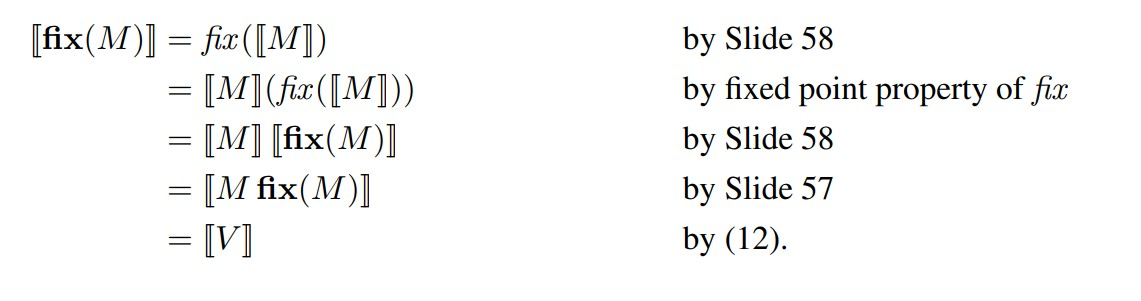
\includegraphics[scale = 0.7]{figs/fix_soundness}
\end{center}
and our code\footnote{Again, this has been manufactured to look similar to the lecture notes, this may disguise various difficulties coercing Agda to play nicely, but proving it did not require any extra mathematical insight, only familiarity with Agda.} mirrors this nicely:
\begin{minted}{agda}
soundness {A} (β-μ {N = N}) =
   begin
     term-⟦ μ M ⟧
   ≡⟨ refl ⟩
     fix-cont ∘ term-⟦ M ⟧
   ≡⟨ cont-fun-extensionality
     (λ x → lfp-is-fixed { ⟦ A ⟧ } {g (mon term-⟦ M ⟧) x })
    ⟩
     ev-cont ∘ pair-f term-⟦ M ⟧ (fix-cont ∘ term-⟦ M ⟧)
   ≡⟨ refl ⟩
     ev-cont ∘ (pair-f term-⟦ M ⟧ term-⟦ μ M ⟧)
   ≡⟨ refl ⟩
     term-⟦ M · (μ M) ⟧
   ∎
\end{minted}
Note that because we use small-step operational semantics, we prove that the denotation of (μ M) is identical of what it reduces to in one step: M · (μ M). The course notes instead have the hypothesis supplied by their big step semantics to justify a final line that equates these to whatever value they reduce to. The interesting step uses the lemma \texttt{lfp-is-fixed}, that the least fixed point of a function is a fixpoint. This is exactly as in the course notes: where this is called the ``fixed point property of \textit{fix}". 

It should also be noted that often in these cases we are trying to prove the equality of two functions, which means we need to use one of three extensionality postulates we have regarding function equality. These all say that functions are equal iff their output is equal for all inputs. We need one each for normal functions from $A$ to $B$, dependent products from $a : A$ to $B(a)$, and continuous functions, from a domain $A$ to a domain $B$. Extensionality is not encoded into Agda but is known to be compatible with it \cite{PLFA}.
\subsubsection{The case of lambdas}
The case of lambdas and applications is one of several examples where things are extremely difficult to formalise, relative to convincing someone with pen and paper. There are approximately three times as many lines of code for proving the lambda case for soundness than all the other cases combined. The lecture notes mention a key substitution lemma, that states that
\[
\llbracket M' [M / x] \rrbracket = \llbracket \tau \vdash M' \rrbracket ( \llbracket M \rrbracket).
\]
We introduce the similar lemma, generalised to terms with arbitrary contexts before them, and altered slightly to fit our code. 

Our lemma is:
\begin{minted}{agda}
substitution-lemma′ : ∀ {Γ} {τ τ′ : Type} → (M : Γ ⊢ τ) → (M′ : Γ , τ ⊢ τ′)
  → ⟦ Γ ⊢′ M′ [ M ] ⟧
     ≡
     ⟦ Γ , τ ⊢′ M′ ⟧ ∘ (pair-f id ⟦ Γ ⊢′ M ⟧)
\end{minted}
The notes claim this can be proven by induction on the structure of $M'$ but this is not so easy. The approach we take, along the lines of Pitts \cite{Pitts} is in fact to define a denotation of substitutions (normally labelled $\sigma$), and then apply that in the case of the single substitution involved in lambdas and prove the two following statements:
\begin{minted}{agda}
comm-triangle : {Γ Δ : Context} {τ : Type} (t : Γ ⊢ τ) 
  → (σ : {A : Type} → Γ ∋ A → Δ ⊢ A)
  → ⟦ Δ ⊢′ subst σ t ⟧ ≡ ⟦ Γ ⊢′ t ⟧ ∘ ⟦ σ ⟧ₛ

lemma-55-corr : {Γ : Context} {τ τ′ : Type} {M : Γ ⊢ τ} {M′ : Γ , τ ⊢ τ′}
  → ⟦ single-sub ⟧ₛ ≡ pair-f id ⟦ Γ ⊢′ M ⟧
\end{minted}
The first is called \texttt{comm-triangle} as it corresponds to the following category-theoretic commutative diagram (CITE). It can be defined by induction on the term \texttt{t}, where, as with many other things, most of the cases are simple and just use the induction hypothesis, but the cases of lambdas and variables are tough and require a few hundred more lines of lemmas justifying each step. The second is a corrolary of what Pitts numbers lemma 5.5, hence its name. With these two theorems, we can prove the substitution-lemma as follows:
\begin{minted}{agda}
substitution-lemma′ {Γ} {τ} {τ′} M M′ =
  begin
    ⟦ Γ ⊢′ M′ [ M ] ⟧
  ≡⟨ comm-triangle M′ single-sub ⟩
    ⟦ Γ , τ ⊢′ M′ ⟧ ∘ ⟦ single-sub ⟧ₛ
  ≡⟨ lemma-55-corr {Γ} {τ} {τ′} {M} {M′}⟩
    ⟦ Γ , τ ⊢′ M′ ⟧ ∘ (pair-f id ⟦ Γ ⊢′ M ⟧)
  ∎
\end{minted}
With this substitution lemma (wherein lies most of the difficulty of the lambda case), we can handle the soundness case for applications of a reduced lambda:
\begin{minted}{agda}
soundness (β-ƛ {A = A} {B} {N} {W}) =
 begin
   term-⟦ (ƛ N) · W ⟧
 ≡⟨ refl ⟩
   ev-cont ∘ pair-f term-⟦ ƛ N ⟧ term-⟦ W ⟧
 ≡⟨ cong (_∘_ ev-cont) (cong (λ x → pair-f x term-⟦ W ⟧) (cont-fun-extensionality (λ x → refl))) ⟩
   ev-cont ∘ (pair-f (cur-cont (⟦ ∅ , A ⊢′ N ⟧)) term-⟦ W ⟧)
 ≡⟨ pair-lemma-corr {A} {B} {N} {W} ⟩
   ⟦ ∅ , A ⊢′ N ⟧ ∘ (pair-f id term-⟦ W ⟧)
 ≡⟨ Eq.sym (substitution-lemma′ W N) ⟩
   term-⟦ N [ W ] ⟧
 ∎
\end{minted}
The first, second and third lines are all able to be shown equal without any sophistry: Agda can recognise the first equality, and the second relies upon congruence and the \texttt{cont-fun-extensionality} postulate but the proof within that is just \texttt{refl}. 

From there, we use a (fairly easy-to-prove) lemma to prove the equality to the fourth term, and finally our substitution lemma for the final term. Note the subtlety of the approach we took: despite the fact that this proof doesn't directly involve a denotation of substitutions, in order to prove the lemmas it uses, we needed this denotation\footnote{In fact, our approach involves giving a denotation to renamings as well. Variables and contexts really are tough to formalise!}. This is in contrast to the ease of stating the appropriate lemmas: though we had to adapt the statement given design decisions (for example, our substitution lemma is not identical to the course notes one), one can look at the equality reasoning and read off the necessary lemmas, but their proofs are non-obvious. 
\chapter{Evaluation}
\section{Work Completed}
I completed all the core goals. There are no holes in my code\footnote{I mean this in the specific Agda sense. That is, every function is fully defined.}, and it all typechecks. I used four postulates. Each has been discussed. Three are known to be acceptable, (those of function extensionality) and the fourth is obviously true in a non-constructive setting; indeed it is used to prove something that the lecture notes deem trivial. 
\subsection{Core}
I completed each core goal; both those about encoding both domain theory generally, and those about PCF and its denotational semantics. Of these, the progress theorem had a very minor complication; it only holds true with a slight modification to PCF's operational semantics. However, this modification is frequently made in the literature \cite{Hart} \cite{De-Jong} and so this was not a particular issue. Of the goals, by far the two largest surprises in difficulty were dealing with flat domains and the soundness lemma.
\subsection{Extensions}
I proposed four potential extensions: of these the first was not very strictly-defined, and of the other three, the adequacy theorem would probably have been the largest extension (or possibly the category-theoretic approach). 

I avoided the category-theoretic approach for two reasons. Firstly, it would have involved talking at a higher level of abstraction, and thus every record would have more fields and I thought this would make the core work (the domain theory content) harder to see below the higher-level abstraction\footnote{Consider if, for example, every function was actually a morphism, and every equality was an equivalence relation, and thus we could not use $\equiv$ and $\lambda$ from Agda, but had to introduce extra symbols throughout.}. This made it unattractive to me, for aesthetic reasons if nothing else. Secondly, the category-theoretic approach to denotational semantics is not very far away from the strategy I used to formalise the proof of the soundness lemma\footnote{Indeed Pitts's work \cite{Pitts} is a work from a series of lectures on category theory.}. This meant that I didn't feel I would be proving much in addition, or gaining extra benefits from the abstraction, as I was already leveraging the category-theoretic viewpoint to help where beneficial. 

I avoided the adequacy proof due to time limitations. I was more or less on-schedule for most of the process, but ended up behind due to how difficult I found the soundness lemma was to prove. I thus judged it safer to aim for smaller extensions, that I was more confident I could complete, than for the adequacy proof and risk having nothing. 
\section{Unit tests?}
Evaluating formalisations is a tricky thing. If one trusts the typechecker, the typechecking is its own evaluation. There is no point writing a unit test to check a theorem is true: the proof is that it typechecks. However, as discussed prior, what is not certain is that the definitions in one's code correspond to the mathematics one claims. We can thus check that with some level of testing. 
\subsection{Our PCF is PCF}
We can check that programs compute the values we think we do. Earlier we presented the factorial function as a use of the fix operator. We can encode this and see what it reduces to. 
\begin{minted}{agda}
add : ∀ {Γ} → Γ ⊢ `ℕ ⇒ `ℕ ⇒ `ℕ
add = μ (ƛ (ƛ (ƛ (if `is-zero (` Z) then ` S Z else (` (S S Z) · `suc ` S Z · (`pred (` Z)))))))

times : ∀ {Γ} → Γ ⊢ `ℕ ⇒ `ℕ ⇒ `ℕ
times = μ (ƛ (ƛ (ƛ (if `is-zero (` Z) then `zero else (add · ` S Z · (` S S Z · ` S Z · (`pred (` Z))))))))

factorial : ∀ {Γ} → Γ ⊢ `ℕ ⇒ `ℕ
factorial = μ (ƛ (ƛ (if `is-zero (` Z) then (`suc `zero) else (times · ` Z · (` S Z · (`pred (` Z)))))))
\end{minted}
Because Agda has a termination checker, we can't just compute things, so we steal an approach from Wadler \cite{PLFA}, where the number of evaluation steps (called ``gas") is pre-specified. This allows us to compute using the IDE's ``convert to normal form" feature. Defining the relevant terms and then typing in for example:
\begin{minted}{agda}
eval (gas 1000) (factorial · (` suc (`suc (`suc `zero))))
\end{minted}
gives us a very long line of reduction steps, followed by 
\begin{minted}{agda}
done (V-suc (V-suc (V-suc (V-suc (V-suc (V-suc V-zero))))))
\end{minted}
That is, we obtain a proof that our evaluation gives a value, and that proof is a proof that 6 is a value, so the evaluation gave 6. So our factorial function seems correct!

More generally with regard to semantics, we earlier claimed that the choice of small-step semantics had no downside (the benefit is that it allows for direct computation). We here present a proof that all the same evaluation rules still hold.

First we define the transitive closure of our small-step semantics:
\begin{multicols}{3}
\begin{minted}{agda}
data _-→*_ : ∀ {Γ} {A} → Γ ⊢ A → Γ ⊢ A → Set where
  refl-→* : ∀ {Γ} {A}
    → {t : Γ ⊢ A}
    → t -→* t
  single : ∀ {Γ} {A}
    → {t  : Γ ⊢ A}
    → {t′ : Γ ⊢ A}
    → t —→ t′
    → t -→* t′
  trans-→* : ∀ {Γ} {A}
    → {t  : Γ ⊢ A}
    → {t′ : Γ ⊢ A}
    → {t″ : Γ ⊢ A}
    → (t -→* t′)
    → (t′ -→* t″)
    → (t -→* t″)
\end{minted}
\end{multicols}
Then we define big-step reduction as a product type, with the first part being a proof that it is a composition of small-step reductions, and the second being a proof that the end term is a value:
\begin{minted}{agda}
_⇓_ : ∀ {Γ} {A} → (M : Γ ⊢ A) → (V : Γ ⊢ A) → Set
M ⇓ V = M -→* V × Value V 
\end{minted}
Then we can define all our theorems, which are the big-step evaluations from the course. That is, we prove they hold according to our definitions, and so our small-step semantics imply the big-step ones:
\begin{minted}{agda}
⇓-Val : ∀ {Γ} {A} {V : Γ ⊢ A} → Value V → V ⇓ V
⇓-succ : ∀ {Γ} {M : Γ ⊢ `ℕ} {V : Γ ⊢ `ℕ} → M ⇓ V → (`suc M) ⇓ (`suc V)
⇓-pred : ∀ {Γ} {M : Γ ⊢ `ℕ} {V : Γ ⊢ `ℕ} → M ⇓ (`suc V) → (`pred M) ⇓ V
⇓-zero₁ : ∀ {Γ} {M : Γ ⊢ `ℕ} → M ⇓ `zero → (`is-zero M) ⇓ `true
⇓-zero₂ : ∀ {Γ} {M : Γ ⊢ `ℕ} {V : Γ ⊢ `ℕ} → M ⇓ (`suc V) → (`is-zero M) ⇓ `false
⇓-if₁ : ∀ {Γ} {A} {M₁ : Γ ⊢ `bool} {M₂ M₃ V : Γ ⊢ A} → M₁ ⇓ `true
  → M₂ ⇓ V → (if M₁ then M₂ else M₃) ⇓ V
⇓-if₂ : ∀ {Γ} {A} {M₁ : Γ ⊢ `bool} {M₂ M₃ V : Γ ⊢ A} → M₁ ⇓ `false 
  → M₃ ⇓ V → (if M₁ then M₂ else M₃) ⇓ V
⇓-cbn : ∀ {Γ} {A} {B} {M₁ : Γ ⊢ A ⇒ B} {M₁′ : Γ , A ⊢ B} {M₂ : Γ ⊢ A} {V : Γ ⊢ B} 
  → M₁ ⇓ (ƛ M₁′) → (M₁′ [ M₂ ]) ⇓ V → (M₁ · M₂) ⇓ V 
⇓-fix : ∀ {Γ} {A} {M : Γ ⊢ A ⇒ A} {V : Γ ⊢ A} → (M · (μ M)) ⇓ V → (μ M) ⇓ V
\end{minted}
The proofs require nothing sophisticated, but do use additional lemmas about congruence and inversion. We here demonstrate some examples of the needed lemmas. The proofs, once the lemmas are established, are all one-liners. 

First, our congruence proofs normally convert small-step congruences to compositions of step congruences. For example, we wish to show that, just as our small-step reduction rule is that if $M$ steps to $N$ then $suc(M)$ steps to $suc(N)$, this holds for bigger steps too. We prove by induction on the proof that $M$ steps to $N$:
\begin{minted}{agda}
cong-suc : ∀ {Γ} {M V : Γ ⊢ `ℕ} → M -→* V → (`suc M) -→* (`suc V)
cong-suc refl-→* = refl-→*
cong-suc (single x) = single (ξ-suc x)
cong-suc (trans-→* x y) = trans-→* (cong-suc x) (cong-suc y)
\end{minted}
Secondly, we sometimes can invert a rule, giving us inversion lemmas. For example, we want to show that if \texttt{`suc V}  is a value, then so too is \texttt{V} while our definition for values says the exact opposite. But we can do induction on the proof that \texttt{`suc V} is a value, and because there is only one constructor, the proof immediately follows:
\begin{minted}{agda}
suc-val-inversion : ∀ {Γ} {V : Γ ⊢ `ℕ} → Value (`suc V) → Value V
suc-val-inversion (V-suc x) = x
\end{minted} 
\subsection{Our denotational semantics are correct}
As well as demonstrating that our operational semantics seem non-problematic, we may try to explicitly calculate the denotations of some interesting closed terms. This is an approach used in other places such as \cite{Hart} \cite{C-DenSem2}, but note that, particularly when dealing with Agda, computational issues are a problem. 

This is true in two senses: firstly, Agda is slow. When dealing with a language within the language, calculations of denotations of quite simple terms can take minutes to compute.

Secondly, we return to the issue of non-constructive lubs on flat domains. The denotation of some terms (notably those involving the fix operator) involves taking a lub of a chain that may or may not be all bottom elements. Earlier, we got around this issue by postulating a constructive proof of the lub of a chain in a flat domain, but now we want to actually compute this lub. To do this, we must disable Agda's termination checker. 

We write a function that looks along the chain, stopping once it gets to a non-bottom element. Of course, this function may not terminate, but for the purposes we wish to use it, this is fine:
\begin{minted}{agda}
{-# TERMINATING #-}
get-lub-in-flat-domain : ∀ {B} → (c : chain (flat-domain-pos B)) → ℕ → B
get-lub-in-flat-domain c n with g c n
...                          | ⊥₁ = get-lub-in-flat-domain c (suc n)
...                          | inj x = x
\end{minted}

Having done this, we can verify some things we expect to be true, like:
\begin{itemize}
\item the denotation of 3. Here indeed we obtain \texttt{inj (suc (suc (suc zero)))} as hoped.
\item the denotation of $2+2$. Here indeed we obtain \texttt{inj (suc (suc (suc (suc zero))))} as hoped.
\item the denotation of $6$ times $3$. I won't write it out, but we do indeed get 18.
\end{itemize}
Note that we are unable to calculate the denotation of our factorial term, but this is nonetheless a partial step forward. Hart \cite{Hart} is unable to verify the denotation of any terms involving the fix operator, while our times function has two nested uses of the fix operator. Similarly, according to Ellison \cite{C-DenSem2} Papaspyrou's system of denotational semantics for C \cite{C-DenSem} is not sufficient to calculate the ``factorial of six or the fourth Fibonacci number". So, validation being computationally hard is a standard issue. 
\section{Agda and Curry-Howard Theorem Proving}
Krishnaswami \cite{Types} writes about using Agda as a theorem prover: ``Writing a program becomes the same as proving it correct. This is hard, like learning to program again! But also extremely fun". This well describes my experience. In much the same way that all programmers write bugs, all mathematicians write false proofs (CITE Wiles, footnote about Mochizuki). But, with Agda, one doesn't need to worry quite so much. While it becomes much harder to prove many of the same things, one's confidence in the proofs rises to near-certainty. 

I was often stunned positively by Agda, seeing it make proofs simpler by doing much of the computation automatically that one would express on paper. Nonetheless, I have serious complaints about Agda that impeded my workflow and progress during this project. In no particular order, I think the most serious were around performance with nested records and difficult-to-understand behaviour around $\eta$-expansion. Firstly, some of my proofs (in particular those around the substitution lemma) had to be type-checked case by case, as checking them all at once was computationally prohibitive. This seems to be a known issue around multiple layers of nesting records (Cite?). These performance issues became more relevant during sanity-checking, testing the denotations of some terms were what one would expect. Secondly, often Agda complains that it fails to solve a unification problem but is capable of solving the same problem just by $\eta$-expanding a function. This leads to hard to understand error messages with surprising solutions, as well as often making code uglier, as it is full of $\eta$-expanded functions, seemingly for no reason. 

Formalising languages is known to have common pain points and a prototypical example involves variables and substitution (Cite other examples). While extrinsic typing and use of string-based variable names make the problems worse, even de Bruijn indices and intrinsic typing are not a panacea. Lemmas that seem straightforward by hand and concepts that seem obvious to explain can be very hard to formalise in a sound and complete way. It often feels like rather than formalising definitions one is more playing a game of trying to convince Agda something that seems obviously true. 
\chapter{Conclusions}
\section{Overview of Results}
This project is essentially a formalisation of Scott's original work \cite{Scott}. While the study of denotational semantics has evolved considerably since Scott initiated it, the majority of the results formalised in this project can be found, sometimes proven, often implied or assumed, in that first paper. In it, Scott defines PCF, gives it a denotational semantics based on continuous functions between domains, and shows important properties that follow, and even defines Scott induction, an extension to my original goals. In his conclusion, he speculates that using his denotational semantics, one could think of ``automating any proof procedure", a foresight of the work that led to Milner's LCF \cite{Milner-LCF} and later, Agda. Nonetheless, I not only have formalised the important results of the paper (as well as those assumed by it), but extended them further and formalised much of the denotational semantics course. In particular, I deal with variables and binding, rather than using the $S$ and $K$ combinators, and I also prove meta-properties about the denotation, such as compositionality.

The initial challenge of the entire project was using Agda as a proof assistant, something with which I had no prior experience. In addition, while some of the arguments involved in the proofs were not so complex to translate, several areas were hard to carry over: these include dealing with substitution, flat domains and the initial formalisation of objects. By far the two largest things-to-change about my approach, retrospectively, involve the time spent dealing with ineffective representations of objects, and the time spent dealing with substitution. By consulting more of the literature, I believe that the latter could have been avoided for the most part \cite{Dima-Soas} \cite{Pitts}, while the former is seems an almost-unavoidable consequence of formalising. A priori, it is very hard to reason about the most effective representations (unless some have obvious downsides), so there is little one can do other than choose one that seems to work, and switch if it fails.

I am very glad of two choices in approach. The first was to use Agda; despite my complaints I found it both incredibly helpful (with good editor support and ability to write code that looks familiar to mathematicians) and satisfying to use: while I had computational problems near the end, the majority of the development process involved me type-checking code and feeling a pleasant sense of relief and progress a millisecond or two later (in the cases it did type check!). The other choice that seemed to be beneficial was the use of de Bruijn indices and intrinisically-typed terms. This idea was mainly a consequence of inspiration by Wadler \cite{PLFA}, but I believed it saved me writing more code, and also made it much easier to reason about the terms I was interested in, by making the uninteresting ones unrepresentable. 
	
Overall, both in my original proposal, and in my subsequent MoSCoW analysis, I laid out what I hoped to achieve. I achieved essentially everything I concluded was necessary (with a slight caveat that my method involving flat domains is to some extent ``cheating"), and two of my proposed four extensions, one of which I classed a ``should have"\footnote{This was Scott induction. It is interesting to note that Scott's original work highlights this as the most novel feature and useful aspect to his PCF and denotational semantics. Despite that, its proof is fairly simple and it is essentially a wrapper around induction on the natural numbers. For this reason, it has not been mentioned in detail.} and the other a ``could have"\footnote{This was compositionality of the denotational semantics. This theorem was very simple to prove in the end, as it follows directly from the definitions and was thus not talked about further.}. 

Evaluating formalised proofs is hard, but of the options available to me, I think my choices were reasonable and my evaluation did give me further confidence in the validity of my results: that not only did the code type check but that it actually did what I thought and wanted it to. Because I achieved my success criteria (as well as two, albeit small, extensions), and because my evaluation makes me believe this success was genuine and not some kind of mirage caused by a mismatch between criteria and actual goals, I believe this project was a success.
\section{Future Work}
When formalising denotational semantics of a language, one can go further in two directions. One can try to prove more things: both about the given semantics, or an extension that satisfies more\footnote{The candidate presented for PCF in both the denotational semantics course \textit{and by Scott's original work} is a property called ``full abstraction".}. Or one can try to formalise a language that is somehow more difficult\footnote{For example Papspyrou \cite{C-DenSem} discusses an attempt at giving C a denotational semantics.}. 
	
More specifically to my project, I formalised large parts of a specific set of lectures and notes accompanying them. However, this leaves the obvious gap of the results not formalised. Most interesting among these to me is the failure of full abstraction and Plotkin's result \cite{Plotkin} that adding one additional denotation of a ``parallel or" term is sufficient to allow full abstraction; a result whose formalisation I cannot find in the literature (CHECK). In addition, I did not cover the logical-relation based proof of adequacy of the denotational semantics in my code. Other formalisations of PCF's denotational semantics such as Hart's \cite{Hart} do. 

The other gap standing out to me is around higher levels of abstraction. Much of domain theory involves universal properties: informally these state that not only does an object satisfy some property, but it does so ``better" than any other. For example, least upper bounds are firstly upper bounds (the \texttt{lub1} property), but also the least such (\texttt{the lub2 property}). Similarly, product types not only give functions to each component (the projection functions), but also to any other type which has functions to the same two components. At the right level of abstraction, these ideas are just the details of the same underlying concept. Another motivator to ``zoom out" is that the soundness theorem for denotational semantics can be proven more generally for any cartesian-closed category\footnote{This is, informally, a class with products and functions and some object that there always exists a function to.} using the same structure of proof. This could be a fruitful area for more work, although note that Crole \cite{Crole} has already done some research in this direction. 
\section{Summary}
In this project I formalised definitions of the main objects of domain theory, proved theorems about these, and used these theorems to formalise the denotational semantics of PCF and prove theorems about this semantics. The main results that stand out from this are proving soundness (with respect to the operational semantics) and compositionality. In addition, the approach presented for dealing with flat domains (while simple, relative to the more advanced mathematical machinery that allows things to work fine constructively) is, to my knowledge, novel in spirit, if not particularly creative. Along with flat domains, substitution provided particularly difficulties, relying upon a category-theory-inspired approach in order to show soundness of substitution. 

This has been lots of fun, and a valuable exercise in formalisation - possibly this material could even be integrated into future years of this course - as well as a demonstration of the usability of modern proof assistants like Agda. 
\bibliography{refs}
\end{document}